% KDB: I included the AIAA-pretty class if you want. Use [journal]{aiaa-pretty} to get it into dual coloumn

\documentclass{AIAA}
%\documentclass[12pt,fleqn]{book}

\usepackage{float}
\usepackage{subfig}
\RequirePackage{amsmath}
\usepackage{graphicx}
%\usepackage{caption}
%\usepackage{subcaption}
\usepackage{units}
\usepackage{siunitx}
%\usepackage{multicol}
\usepackage{makecell}
\usepackage{hhline}
\usepackage{wasysym} %For diameter symbol \diameter
\usepackage{tikz} % For fbox amongs others?
\usepackage[export]{adjustbox} % for valign

%% Following packages for commenting modifications:
\usepackage{soul}
\usepackage{color}
\usepackage{setspace}

%You can also define your own mathematics shorthands
\newcommand{\diff}{\mbox{\,d}}
\newcommand{\grad}{\mbox{$\nabla$}}
\newcommand{\divg}{\mbox{$\nabla\cdot\,$}}
\newcommand{\rot}{\mbox{$\nabla\times$}}
\newcommand{\pdiff}{\mbox{$\,\partial$}}

\newcommand{\degr}[1]{\mbox{#1$^o$}}

\newcommand{\slfrac}[2]{\left.#1\middle/#2\right.}

%\newcommand*\circled[1]{\tikz[baseline=(char.base)]{
%            \node[shape=circle,draw,inner sep=1pt] (char) {#1};}}
            
%The following newcommand allow to add a line break within a table cell using \specialcell{Something\\Something}            
\newcommand{\specialcell}[2][c]{%
\begin{tabular}[#1]{@{}c@{}}#2\end{tabular}}

\begin{document}


\title{Experimental and Numerical Heat Transfer from Vortex-Injection Interaction in Scramjet Flowfields}

\author{Juan R. Llobet\footnote{PhD candidate, Centre for Hypersonics, School of Mechanical and Mining Engineering, j.r.llobet@uq.edu.au, Student Member AIAA.}, Kevin D. Basore\footnote{PhD candidate, Centre for Hypersonics, School of Mechanical and Mining Engineering, k.basore@uq.edu.au, Student Member AIAA.}, Rowan J. Gollan\footnote{Lecturer, Centre for Hypersonics, School of Mechanical and Mining Engineering, r.gollan@uq.edu.au, Member AIAA.} and Ingo H. Jahn\footnote{Lecturer, Centre for Hypersonics, School of Mechanical and Mining Engineering, i.jahn@uq.edu.au, Member AIAA.}}
\affiliation{University of Queensland, Brisbane, QLD 4072, Australia}

\begin{abstract}


Air-breathing propulsion is expected to decrease the cost per kilogram for access-to-space while increasing the flexibility of available low earth orbits.
However, improvements are required in order make this a reality, with one of the current issues under investigation being the effective fuel-air mixing inside of scramjet engines.
A viable option suggested to address this issue uses the intrinsically generated vortices from scramjet inlets to enhance the downstream fuel-air mixing.
Previous works have studied this vortex-injection interaction numerically, but the lack of published experimental data in the hypersonic regime made validation impractical.
This paper extends upon these previous works by providing experimental data for the canonical geometry and assessing the numerical methodology to accurately predict the vortex-injection interaction.


To achieve this, an experimental model consisting of a flat plate with a perpendicular compression fin and a porthole injector was tested in the T4 Stalker Tube.
The experimental data recorded was replicated numerically, allowing for the validation of the numerical methods.
These results showed a localized overprediction of the heat transfer, attributed to a localized overprediction of the turbulent kinetic energy.
Nonetheless, a good agreement was seen overall between the numerical and experimental results. 


\end{abstract}

\maketitle

 \section*{Nomenclature}
% (Nomenclature entries should have the units identified)\\
 \noindent\begin{tabular}{@{}lcl@{}}
\textit{$\diameter$}  &=& Diameter $[\SI{}{\milli\meter}]$\\
\textit{$\alpha_{fin}$}  &=& Fin angle $[\SI{}{\deg}]$\\
\textit{$\alpha_R$}  &=& TFHG sensitivity $[\SI{}{\per\kelvin}]$\\
\textit{$\delta$}  &=& Boundary layer thickness $[\SI{}{\milli\meter}]$ \\
\textit{$\rho$}  &=& Density $[\SI{}{\kilo\gram\per\cubic\meter}]$\\
\textit{$c$}  &=& Thermal capacity $[\SI{}{\joule\per\kilo\gram\kelvin}]$ \\
\textit{$H$}  &=& Enthalpy $[\SI{}{\mega\joule\per\kilo\gram}]$\\
\textit{$k_T$}  &=& Thermal conductivity $[\SI{}{\watt\per\meter\kelvin}]$ \\
\textit{M}  &=& Mach number $[-]$\\
\textit{$P$}  &=& Pressure $[\SI{}{\pascal}]$\\
\textit{$q,\,Q$}  &=& Heat flux $[\SI{}{\kilo/watt/per/square/meter}]$\\
\textit{$t$}  &=& Time $[\SI{}{\second}]$\\
\textit{$T$}  &=& Temperature $[\SI{}{\kelvin}]$\\
\textit{$u$}  &=& Velocity $[\SI{}{\meter\per\second}]$ \\
\textit{$V$}  &=& Voltage $[\SI{}{\volt}]$ \\
 \end{tabular} \\


%%%%%%%%%%%%%%%%%%%%%%%%%%%%%%%%%%%%%%%%%%%%%%%%%%%%%%%%%%%%%%%%%%%%%%%%%%%%%
\section{Introduction}

By removing the requirement of having to carry the propellant oxidizer, air-breathing propulsion has significant theoretical advantages over rockets.
These advantages include, a higher specific impulse, efficiency, and payload mass fraction~\cite{SmartTetlow,CookHueter}.
For these reasons, using air-breathing propulsion for access-to-space missions has the potential to increase the overall efficiency as well as decrease the cost per kilogram of placing satellites into orbit.
However, several aspects of scramjet technology still require substantial improvements prior to scramjet propulsion for access-to-space being considered operational.
The extremely short residence times to mix and burn the fuel within these engines is one of the main challenges.
A previously suggested strategy to enhance mixing while incurring a minimal total loss increase, is to use the vortices intrinsically generated by scramjet inlets.
Non-axisymmetric inlets inherently generate vortices due to the Shock-Wave Boundary-Layer Interactions (SWBLI) present~\cite{Alvi} and have been shown to produce improvements in mixing~\cite{SpacePlanes_paper2015,Llobet_PlumeElongation}.
Llobet et al.~\cite{Llobet_PlumeElongation} was able to show, using a RANS computational fluid dynamics (CFD) study, that by injecting into an approximated inlet sidewall SWBLI vortex, the air-fuel mixing rate was substantially improved.
The vortices in this study were generated using a canonical geometry consisting of a flat plate and a compression wall, which was previously shown to generate vortices representative of those found in scramjet flowfields~\cite{AFMCpaper2014}.
This geometry is replicated in this experiment to provide experimental data as a validation benchmark against the numerical studies previously published on this topic.
These experiments were carried out in the T4 Stalker Tube at the University of Queensland (UQ).



%%%%%%%%%%%%%%%%%%%%%%%%%%%%%%%%%%%%%%%%%%%%%%%%%%%%%%%%%%%%%%%%%%%%%%%%%%%%%
\section{T4 Reflected Shock Tunnel}
	\label{sec:T4Literature}
	
The T4 Stalker Tube is a free-piston reflected shock tube at the University of Queensland. 
Commissioned in 1987~\cite{Doherty:PhD_Thesis_Scram_M10} from the design of Stalker~\cite{Stalker1966}, the tunnel is capable of a total enthalpy range of 3-15 MJ/kg ~\cite{Doherty:PhD_Thesis_Scram_M10} at a variety of different Mach numbers~\cite{Tanimizu:Phd_Thesis}.
This high-enthalpy impulse facility is usually run in a direct connect~\cite{Kirchhartz:PhD_Thesis_Boundary_Combustion, RidingsAndrewNoel2015Iops} or semi free-jet configuration~\cite{Chan:Boundary_Layer_Combustion_Perturbation, Wise_Thesis} due to the relatively small core size of the facility~\cite{Itoh1999, Stalker_2005}.


Able to achieve test times on the order of 1 ms \cite{Stalker_2005}, this facility has been used extensively for scramjet propulsion/high-speed aerodynamic research~\cite{Hunt2009, Wise2014b}.
Figure~\ref{fig:T4_Overview} shows an generic overview of the facility with reference~\cite{Doherty:PhD_Thesis_Scram_M10} containing an extensive description of the facility for the interested reader.

\begin{figure}[h]
\centering
	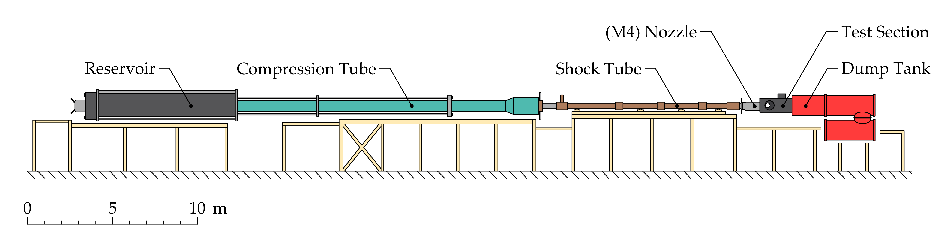
\includegraphics[trim = 0mm 0mm 0mm 0mm, clip, width=0.9\columnwidth]{Figures/T4_Shock_Tunnel_Luke_D_2013.eps}
	\caption{A generic overview of the T4 Stalker Tube. Extracted from ~\cite{Doherty:PhD_Thesis_Scram_M10}.}
	\label{fig:T4_Overview}	
\end{figure}


%%%%%%%%%%%%%%%%%%%%%%%%%%%%%%%%%%%%%%%%%%%%%%%%%%%%%%%%%%%%%%%%%%%%%%%%%%%%%
\section{Experimental Model}
	\label{sec:ModelDescription}

Figure ~\ref{fig:Vortex_Sketches} shows the simplified geometry consisting of a flat plate and a normal fin at an angle of attack used to generate the scramjet-inlet like vortices.
The resulting flowfield, with the freestream velocity moving in the positive x direction, generates a vortex through shock-viscous interactions similar to the vortices generated by non-axisymmetric scramjet inlets~\cite{Llobet_PlumeElongation,AFMCpaper2014}.

\begin{figure}[h]
\center
	\subfloat[Vortex formation and fuel plume]{
	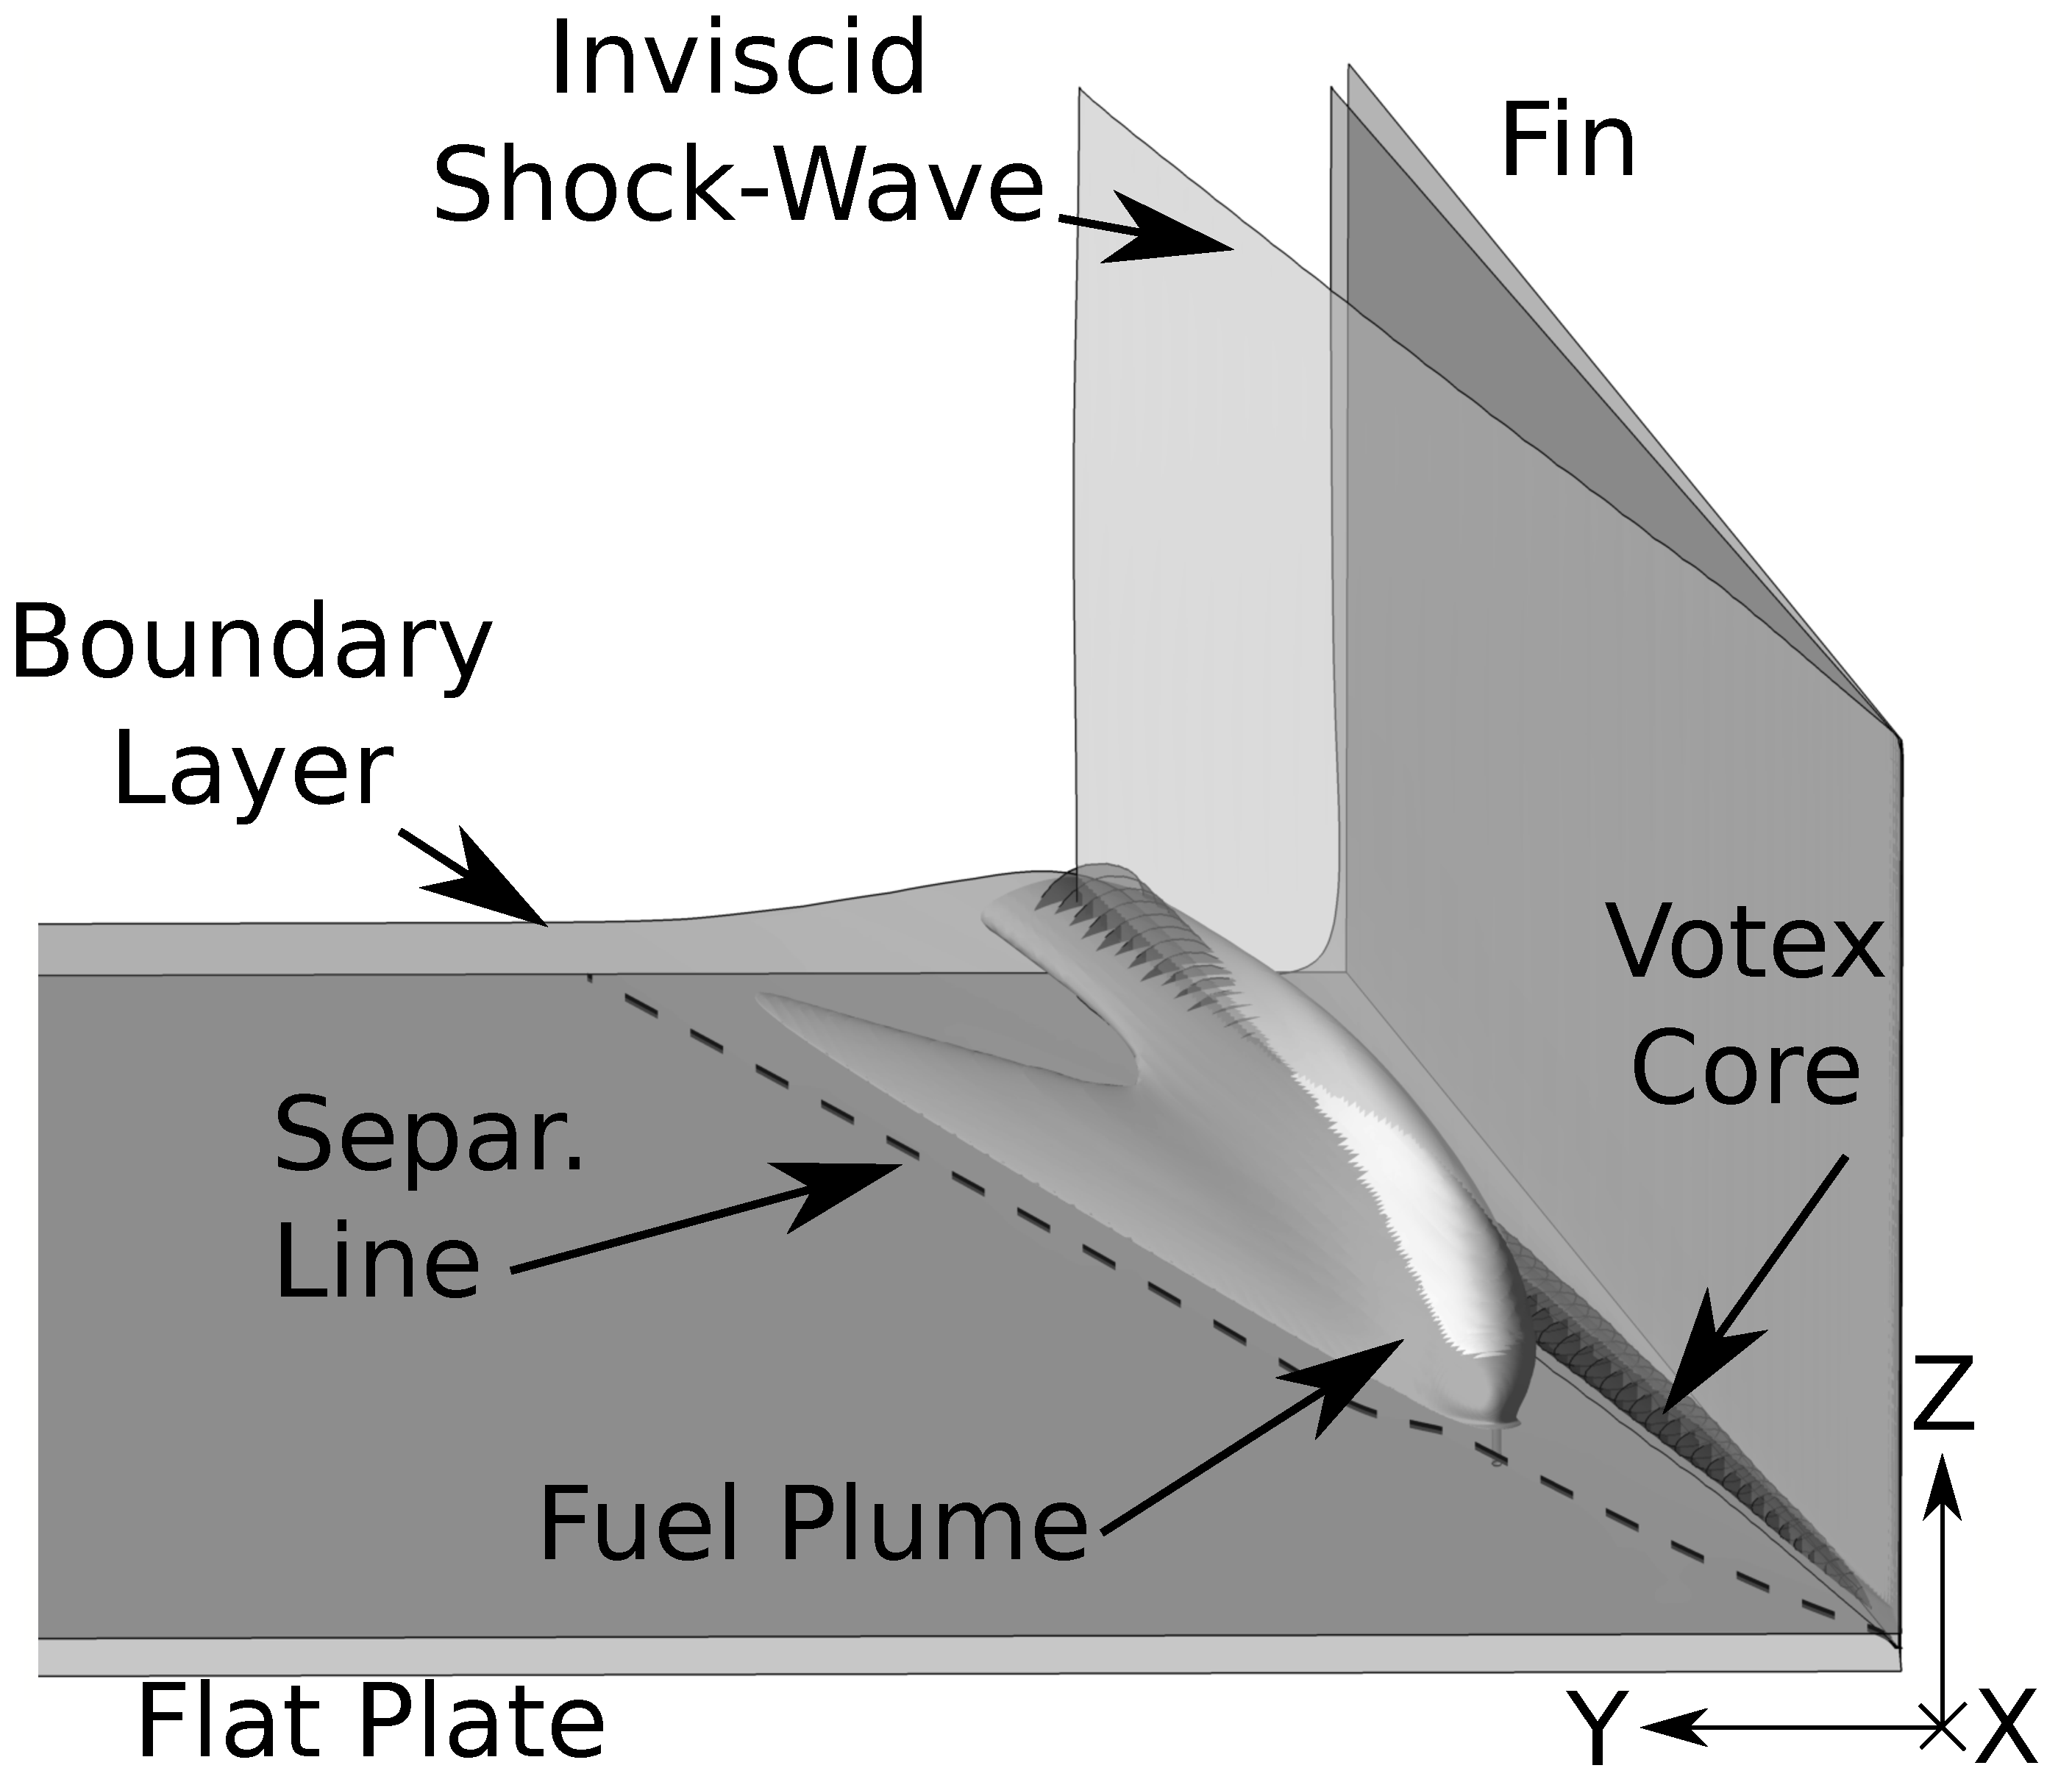
\includegraphics[trim = 0mm 0mm 0mm 0mm, clip, width=0.45\columnwidth]{Figures/Flow_features_V3_B&W.pdf}
	\label{fig:InvShock_BL_Plume}
	}
	\subfloat[Vortex flowfield structure. $\delta$ and contours from  $\alpha_{fin} = 10$ case. Discontinuous lines are adapted from Alvi and Settles~\cite{Alvi}.]{
	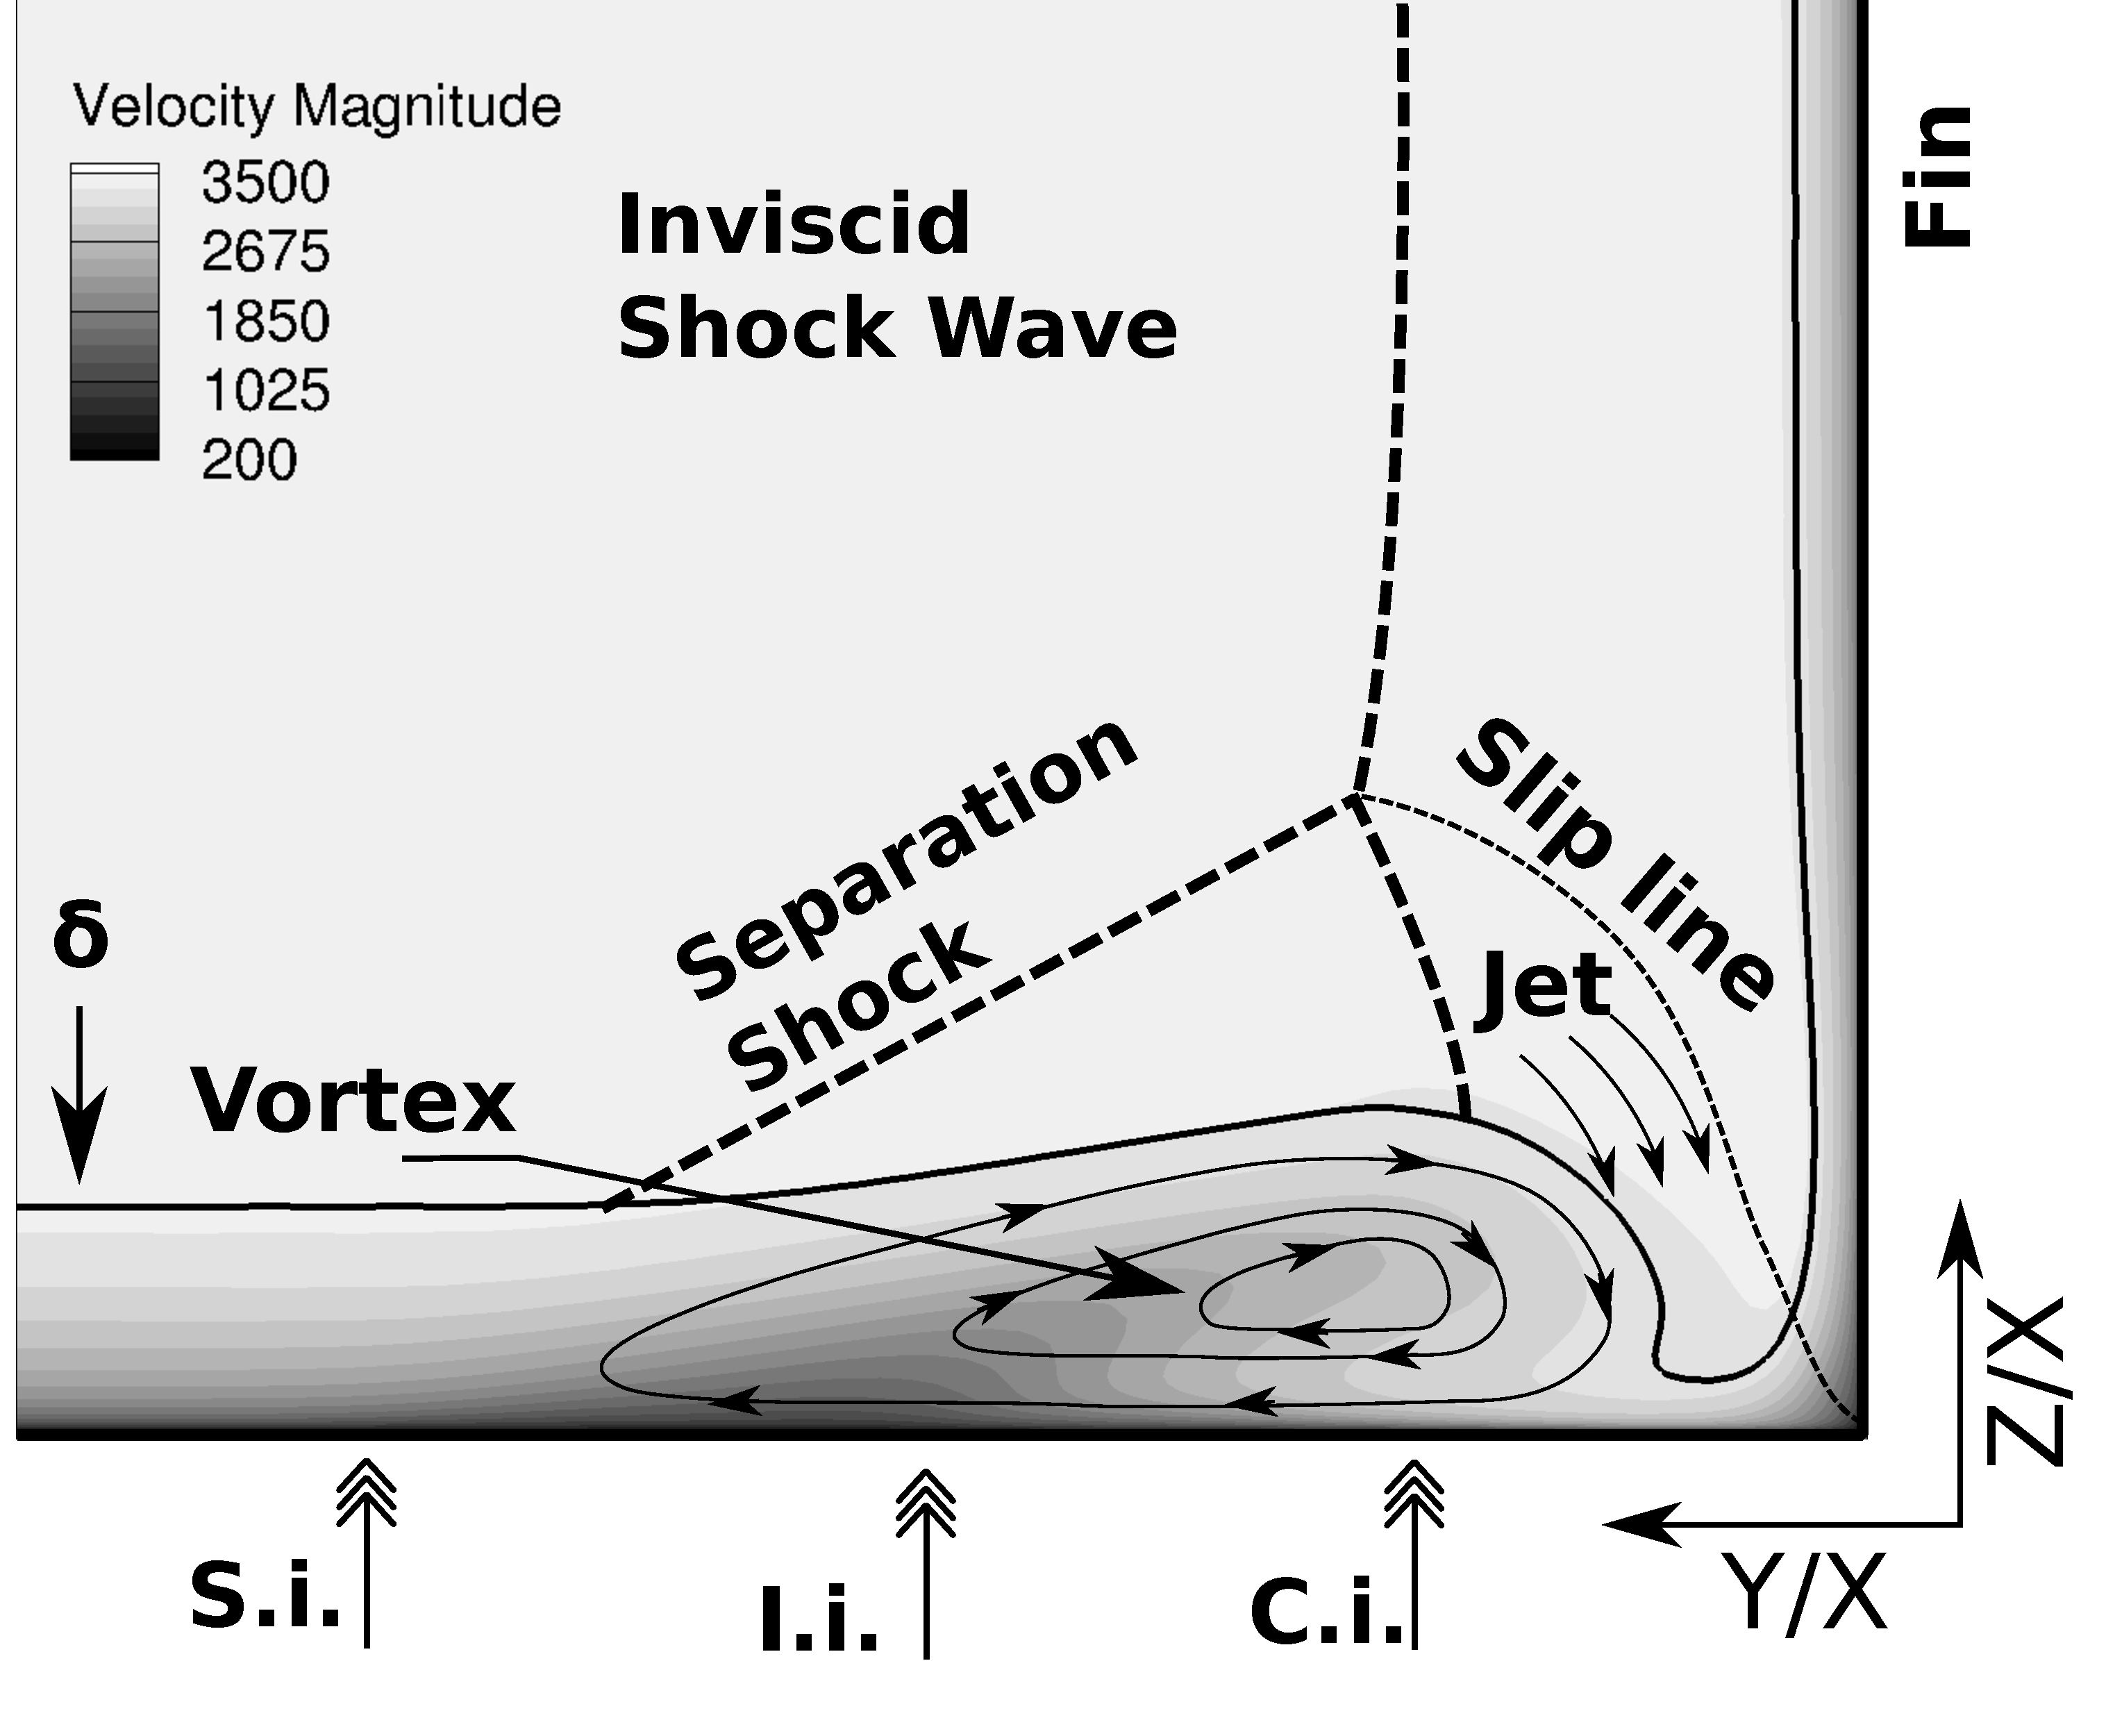
\includegraphics[trim = 2mm 0mm 0mm 2mm, clip, width=0.45\columnwidth]{Figures/AlviSettles_FlowStructure_V5.pdf}
	\label{fig:Alvi_Sketch}
	}
\caption{Test geometry and vortex flowfield structure depiction. Extracted from~\cite{JSASS_paper}}  
\label{fig:Vortex_Sketches}	
\end{figure}


% KDB: Temp formatting to make it more readable.
\hfill\newline


Shown in Fig.~\ref{fig:ModelPics}, the geometry used in the experimental testing is similar to the one used in previous numerical studies~\cite{SpacePlanes_paper2015,AFMCpaper2014,JSASS_paper,Llobet_PlumeElongation}.
For the experimental testing the fin angle was set at \ang{10}.
This angle was chosen due to the relative strength of the vortex generated being representative of the vortices present in previously tested engines~\cite{AFMCpaper2014,SpacePlanes_paper2015}.

%
\begin{figure}[!h]
\center
\subfloat[Model picture.]{
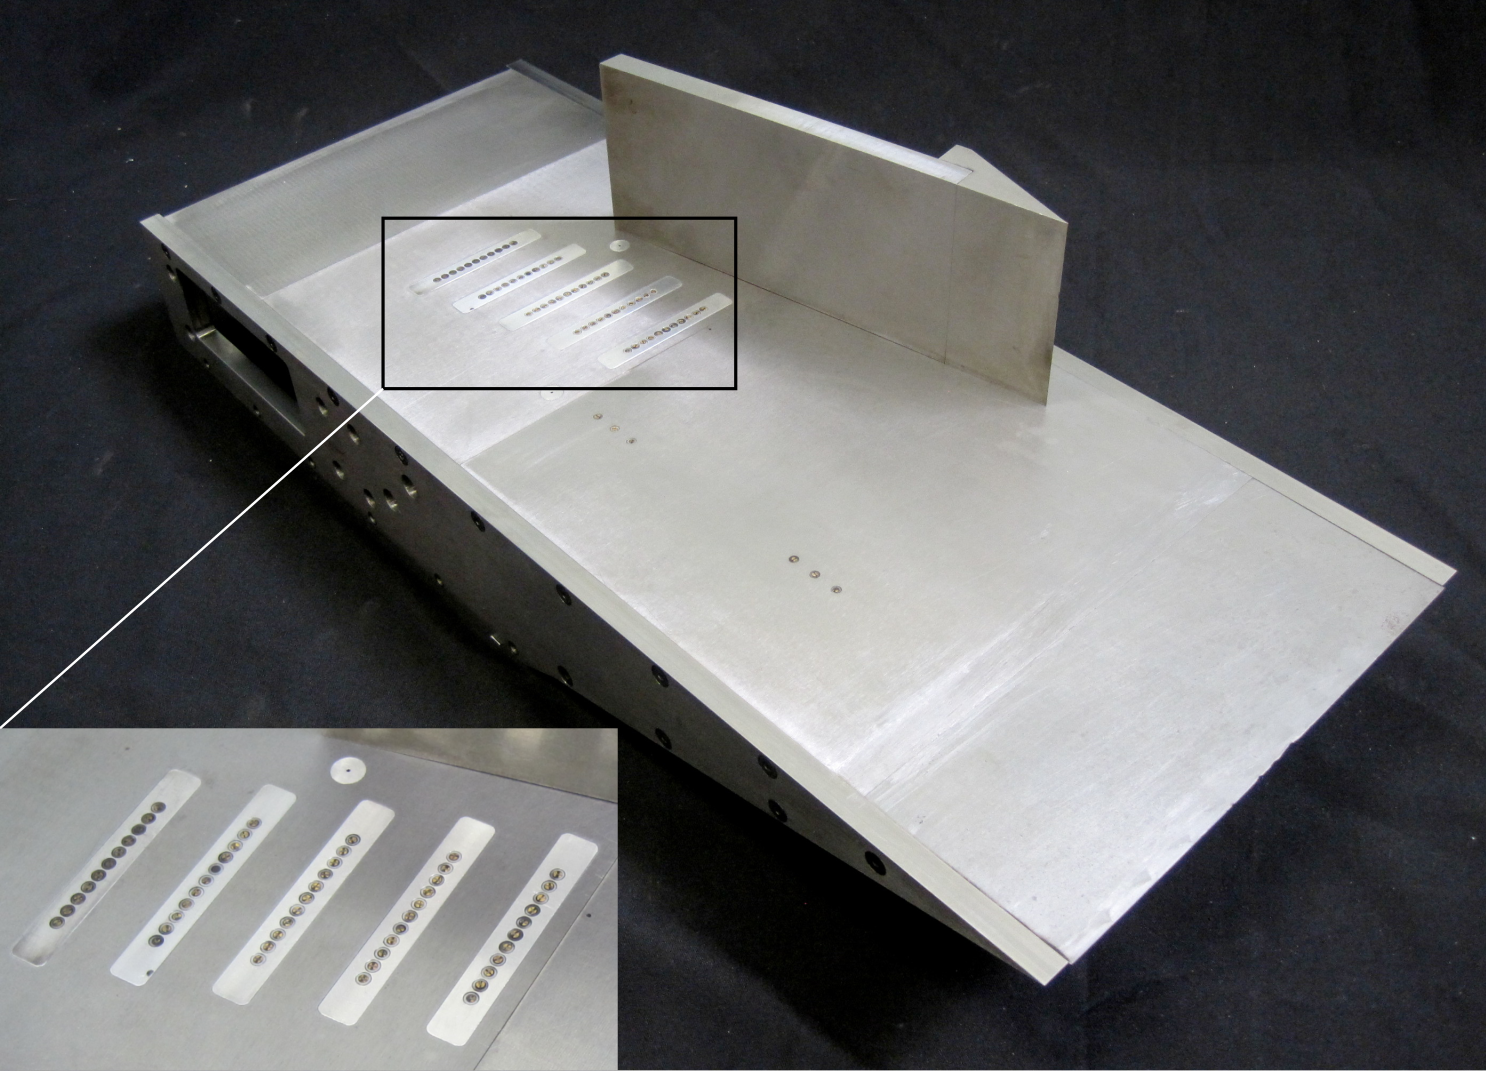
\includegraphics[width=0.50\columnwidth]{Figures/Model_and_zoom.png}
\label{fig:ModelPicture}
}
\subfloat[Detail of gauges distribution location.]{
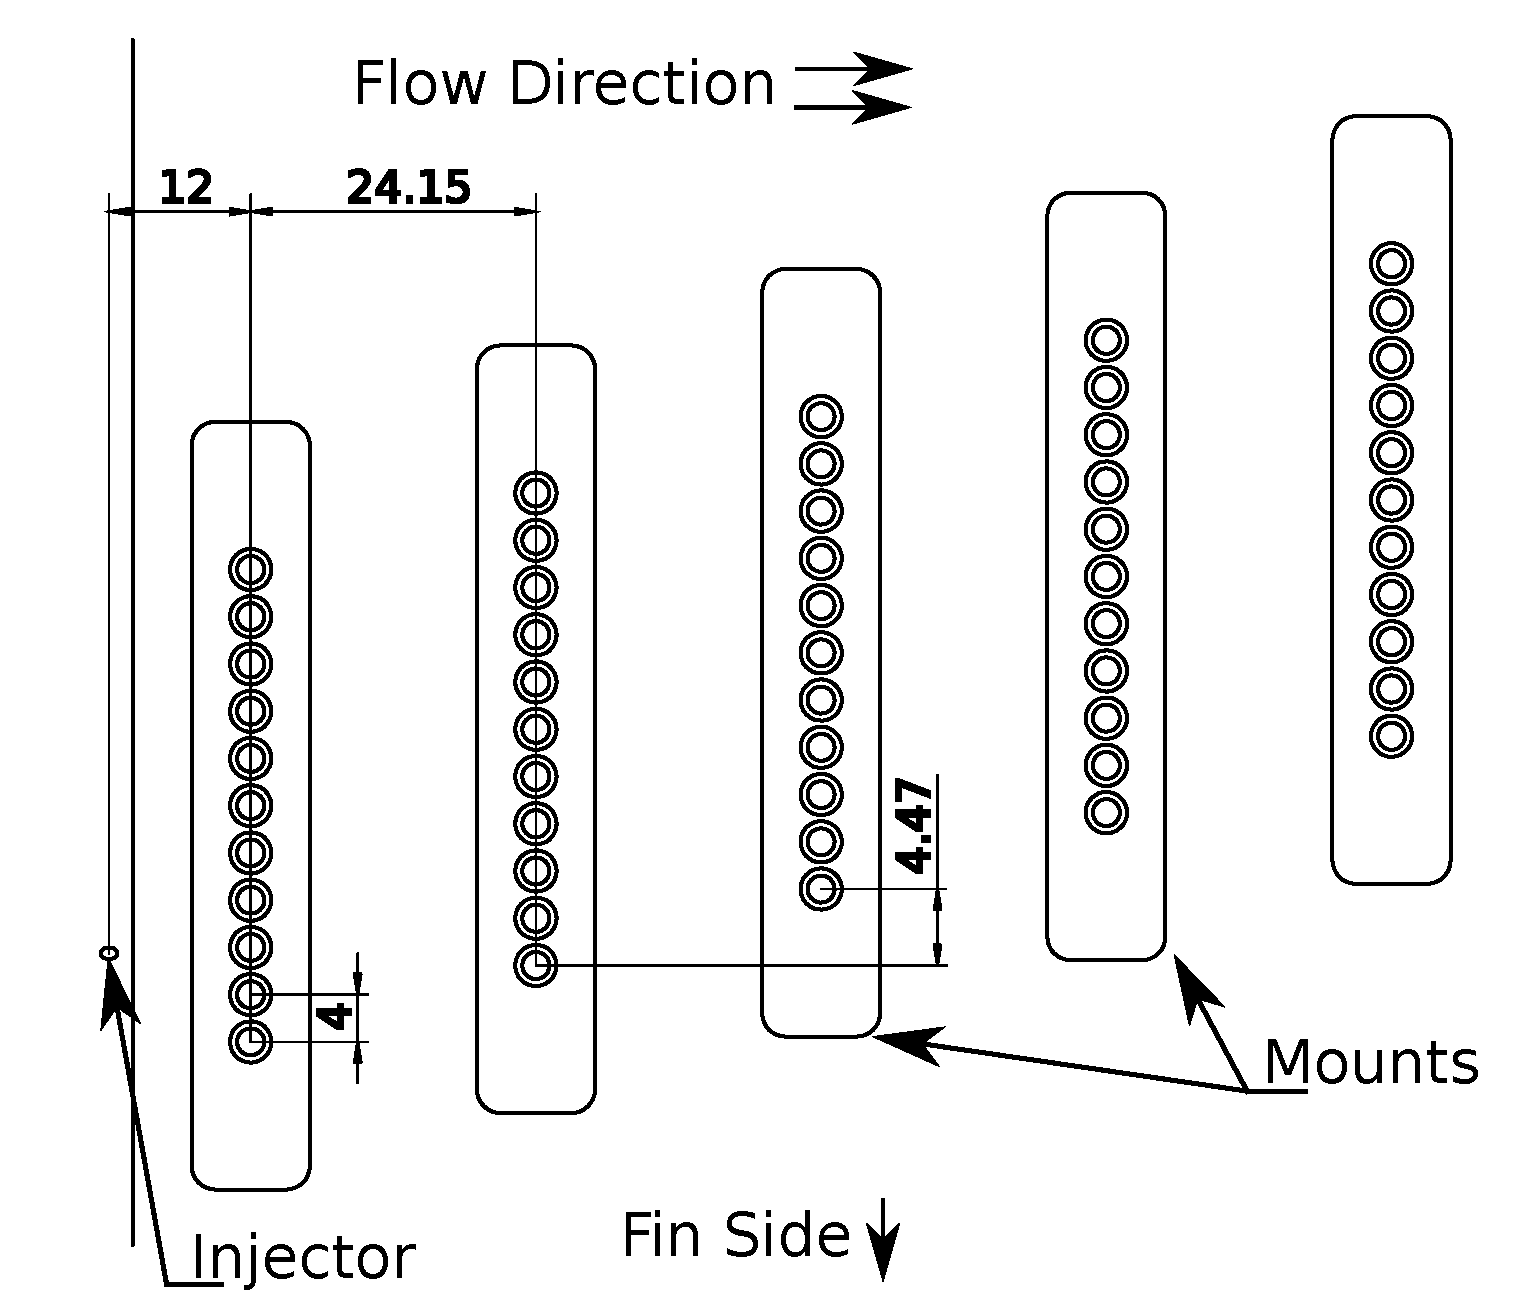
\includegraphics[width=0.40\columnwidth]{Figures/Mounts_Drawing.pdf}
\label{fig:GaugesonModel}
}
\caption{Experimental model in its two configurations.}
\label{fig:ModelPics}
\end{figure} 


The width of the model/plate is $\SI{220}{\milli\meter}$ and was selected to reduce the potential of any three-dimensional effects contaminating the sensor field.
The length of flat plate upstream of the fin leading edge was limited to $\SI{156}{\milli\meter}$ due to the potential interference with the tunnel nozzle walls.
%The location of the fin and injector were adapted for the experimental testing, when compared to the previous numerical configuration, to accommodate the optical constraints of the T4 test section.
The $\SI{1}{\milli\meter}$ diameter injector was located $\SI{126}{\milli\meter}$ downstream of the fin leading edge at a $\SI{45}{\deg}$ angle relative to the freestream flow.
Shown in Fig.~\ref{fig:GaugesonModel}, the fin can be translated in the model Y axis
which allows for different vortex injection locations to be examined. 

The Thin-Film Heat-transfer Gauges (TFHG) in the model were arranged in five parallel lines as shown in the subset of Fig.\ref{fig:ModelPicture}.
Each of the gauge lines contains 11 TFHGs that were manufactured at the Centre for Hypersonics.
These gauges are made using an $\approx$\SI{20}{\nano\meter} nickel resistive strip element that is sputtered onto an optically smooth quartz substrate.
Shielded with a layer of $SiO_2$, the gauges are individually calibrated after manufacturing ~\cite{Wise_Thesis}.
Once mounted into the experimental model, the heat flux can be calculated using the integrated measured change in the TFHG voltage from a constant current circuit using Eq.~\ref{eq:TFHG_Heat}, from~\cite{Wise_Thesis,Schultz_Book}, where $\rho c k_T$ is the properties of the substrate and $\alpha_R$ is the resistance-independent calibrated TFHG sensitivity.

\begin{equation}
\dot{q}_n = \frac{\sqrt{\rho c k_T}}{\sqrt{\pi}\alpha_R V_0}\sum^n_{i=1}\frac{V\left(t_0\right)-V\left(t_{i-1}\right)}{\left(t_n-t_i\right)^{1/2}+\left(t_n-t_{i-1}\right)^{1/2}}
\label{eq:TFHG_Heat} 
\end{equation}



Figure~\ref{fig:GaugesonModel} also shows the TFHG sensor field that was required in order to appropriately resolve the heat-transfer profile across the injection-vortex interaction.
The centers of the gauges are separated by $\SI{4}{\milli\meter}$ in the Y axis, while the lines are separated by $\SI{24}{\milli\meter}$ in the X axis (or freestream direction).
Moreover, the gauge lines have a \SI{4.5}{\milli\meter} offset in the positive Y direction in order to improve the sensor coverage.
The first TFHG line is $\SI{12}{\milli\meter}$ downstream of the injector.


Additionally, the model incorporates six TFHG on the opposite side of the  flat plate to the fin as shown in Fig.~\ref{fig:ModelPicture}.
These gauges are used to measure and identify the state of the boundary layer in the vicinity of the fin leading edge and injection location.
These gauges are grouped in two sets of three $\SI{10}{\milli\meter}$ apart with the 
the first set starting at $\SI{143}{\milli\meter}$ from the flat plate leading edge.
This first group is centered at the same axial location as the fin leading edge in order to determine if the BL was laminar before the start of the vortex.
The second set of gauges starts $\SI{249}{\milli\meter}$ downstream of the flat plate leading edge and is located just upstream of the injector.
These gauges are located far enough away from the fin that there is no chance that the resulting shock-wave and vortex could influence the data.
The boundary layer was found to remain laminar for all test conditions presented in this paper.

Two pressure tabs on the flat plate surface incorporating kulite pressure transducers were used to ascertain the pressure of the nozzle exit conditions.



%%%%%%%%%%%%%%%%%%%%%%%%%%%%%%%%%%%%%%%%%%%%%%%%%%%%%%%%%%%%%%%%%%%%%%%%%%%%%
\subsection{T4 test flow conditions}

The experiments were performed using the T4 Mach 7.6 nozzle at a Mach 8 flight-enthalpy.
The nozzle exit flow conditions are derived from measurements of the shock tube fill pressure $\left(P_{ST}\right)$, shock tube shock-speed $\left(u_{S}\right)$, shock tube temperature $\left(T_{ST}\right)$, and the stagnation region nozzle supply pressure $\left(P_e\right)$.
Shown in Table~\ref{tab:Exper_Flow_Cond} is the calculated nozzle exit values tabulated along with their uncertainties.


\begin{table}[!h]
\centering
\caption{Nominal conditions during testing a nozzle exit.}
\label{tab:Exper_Flow_Cond}
\begin{tabular}{rl|rl}
\multicolumn{2}{c|}{Variable} & \multicolumn{2}{c}{Value}\\
\hline
\Gape[0.2cm][0.0cm]{$P_0$} & $[\SI{}{\mega\pascal}]$		& $15.7$ 	& $\pm 4.42\%$ \\
$P_\infty$ 		& $[\SI{}{\kilo\pascal}]$				& $2.29$ 	& $\pm 4.53\%$  \\
$T_\infty$ 		& $[\SI{}{\kelvin}]$						& $237$ 	& $\pm 7.37\%$ \\
$\rho_\infty$	& $[\SI{}{\kilo\gram\per\cubic\meter}]$	& $0.0335$ 	& $\pm 6.97\%$ \\
$u_\infty$ 		& $[\SI{}{\meter\per\second}]$			& $2340$	& $\pm 2.98\%$ \\
$M_\infty$ 		& $[-]$									& $7.57$ 	& $\pm 0.70\%$ \\           
$H_0$ 			& $[\SI{}{\mega\joule\per\kilo\gram}]$	& $2.73$ 	& $\pm 7.10\%$ \\          
\hline
\end{tabular}
\end{table}


The nozzle exit conditions shown in Table~\ref{tab:Exper_Flow_Cond} are calculated using the in-house code NENZFr from the University of Queensland~\cite{nenzfr_manual}.
NENZFr is a wrapper that integrates an ESTCj(\textbf{[ref]}) shock-tube simulation into a space-marched thermal and chemical non-equilibrium Eilmer3 CFD simulation of the nozzle.
Eilmer3 is a collection of programs simulating 2-D/3-D thermal and chemical non-equilibrium transient Navier-Stokes that is also developed at the University of Queensland~\cite{Eilmer_TheoryBook,Eilmer3UserGuide}.


The axisymmetric grid used for the space-marched Eilmer3 simulation is constructed by inscribing a uniform structured grid between a Bezier curve defining the nozzle wall and the nozzle centerline.
The mesh employed in this study consisted of 600 by 40 elements in the axial and radial directions respectively.
The chemical composition of the gas is calculated using finite-rate reactions with a five species air model: $N_2$, $O_2$, $NO$, $N$ and $O$.
The thermodynamic properties are obtained using NASA CEA2~\cite{CEA2,Eilmer_TheoryBook}.

Moreover, to improve the accuracy of the nozzle exit conditions an iterative convergence was applied to the transition location in the nozzle.
The baseline predictive value was iterated upon until a satisfactory convergence was found with the experimentally measured static pressure on the plate.
The uncertainty of this measurement is lower than the resultant sensitivity from the nozzle transition location, and thus is considered a truth value target for the iterative convergence\cite{Doherty:PhD_Thesis_Scram_M10}.


%%%%%%%%%%%%%%%%%%%%%%%%%%%%%%%%%%%%%%%%%%%%%%%%%%%%%%%%%%%%%%%%%%%%%%%%%%%%%
\section{Test cases}

Two fin locations in the model Y axis were examined as a part of the experimental campaign.
Both of these locations corresponded to different relative injection locations in the vortex in order to verify how the effusing fluid influenced the resulting flowfield.
% KDB: I think you need to show this. Remove if you don't want.
%%%%The approximate locations relative to the induced vortex are shown on Fig. \ref{fig:Alvi_Sketch}.
These locations were measured as the perpendicular distance to the fin in the model Y axis  non-dimensionalized by the jet diameter.
The corresponding fin-to-injector distance ratios tested were $26.2\diameter_{inj}$ and $35.2\diameter_{inj}$, and are named the Upper Fin (UF), and Lower Fin (LF) test cases respectively.


Hydrogen was used as the injection fluid for this campaign and was tested at two different plenum pressures at both of the UF and LF locations.
The two pressures tested were $P_{inj}=\SI{1300}{\kilo\pascal}$ and $P_{inj}=\SI{430}{\kilo\pascal}$ and are named the High Injection (HI) and Low Injection (LI) cases respectively.
These two pressures produce injection-to-freestream momentum ratios of $5.24$, and $1.73$ with a Ludwieg tube used in order to maintain a constant total plenum pressure.
The case of No Injection (NI) was used to obtain the baseline undisturbed vortex heat flux data.


All of these parameters were combined to produce six different test cases as summarized in Table~\ref{tab:T4_Test_Cases}.

\begin{table}[!h]
\centering
\caption{Combination of injection pressure and fin position for the different test cases.}
\label{tab:T4_Test_Cases}
\begin{tabular}{lc|c|c}
	$\#$ & Naming  & Injection Pressure & \specialcell{Fin-to-injector\\distance ratio}\\
\hline
\Gape[0.2cm][0.0cm]{1} & NI-UF & - (-) &  $26.2$\\
2 & NI-LF & - (-) &  $35.2$ \\
3 & HI-UF & $\SI{1300}{\kilo\pascal}$ $\pm\SI{3.1}{\percent}$ &  $26.2$ \\
4 & LI-UF & $\SI{430}{\kilo\pascal}$ $\pm\SI{2.8}{\percent}$ &  $26.2$ \\
5 &	HI-LF &  $\SI{1300}{\kilo\pascal}$ $\pm\SI{3.1}{\percent}$ &  $35.2$ \\
6 & LI-LF & $\SI{430}{\kilo\pascal}$ $\pm\SI{2.8}{\percent}$ &  $35.2$ \\

\hline
\end{tabular}
\end{table}


%%%%%%%%%%%%%%%%%%%%%%%%%%%%%%%%%%%%%%%%%%%%%%%%%%%%%%%%%%%%%%%%%%%%%%%%%%%%%
\section{CFD reference results}
\label{sec:CFDReferenceRes}

The data obtained in the experiments is complemented with numerical simulations to enhance the understanding of the results and assess the validity of the numerical methodology.
The numerical domain used spans from $\SI{10}{\milli\meter}$ upstream to $\SI{300}{\milli\meter}$ downstream of the fin leading edge and $\SI{200}{\milli\meter}$ centered around the injector centroid in the spanwise direction.
The boundary layer development over the first $\SI{146}{\milli\meter}$ of the flat plate upstream of the fin leading edge was calculated in a separate quasi two-dimensional simulation with an infinitely sharp leading edge. 
The resulting exit profile from this simulation was input as an infinite plane into the three-dimensional numerical domain described above.

The structured three-dimensional domain contained approximately four million cells and had a minimum spacing around the injector of approximately $\SI{0.05}{\milli\meter}$.
The cell growth from the injector was restricted to $\SI{1}{\milli\meter}$ in the region of uniform flow and was considered a far-field approximation from the vortex-injection interaction.
Inside the numerical domain, the injector was placed at $X=\SI{125}{\milli\meter}$ downstream of the fin leading edge and 26.2 and 35.2 fin-to-injector distances ratios in order to match the experiments.
The walls were modeled as non-slip isothermal with a temperature at $\SI{300}{\kelvin}$, the mean for the lab in which the experiments were conducted. 


The inflow conditions used for the simulations are the nominal conditions calculated at the nozzle exit in Table~\ref{tab:Exper_Flow_Cond}.
Using the transition predictions for the T4 tunnel from He and Morgan~\cite{He_Morgan}, the plate was expected to stay fully laminar upstream of the oblique shock and injector.
Thus, the pseudo-2D simulations were conducted as fully laminar and no boundary layer parabolic stability transition prediction was used. 

The turbulence model used was an SST $k-\omega$ to allow for a more accurate turbulent mixing of the fuel and the production of turbulence in the boundary layer region separated by the fin shock.
In order to accommodate the laminar inflow from the quasi-2D simulation, the 3D domain inflow Turbulent Kinetic Energy (TKE) was set to zero.
By setting this value to zero, the laminar nature of the flow upstream of the fin, as seen in the experiments, was able to be replicated for most of the flat plate.
More importantly, using a zero TKE inflow with the SST $k-\omega$, allowed for an appropriate modeling of the viscous turbulence generation in the laminar boundary layer interaction with the fin shock as well as the separations and injection-vortex interaction.
This TKE generation can be seen in Fig.~\ref{fig:TurbKinEn_CFD_SliceLow} with the one dimensional extraction slice taken along the line displayed in the figure.
Examining this subset extraction in Fig.~\ref{fig:TurbKinEn_CFD_SliceLow}, the TKE remains almost negligible in the initial part of the domain until a rapid onset just downstream of the injector.
Thanks to the delayed onset of TKE growth, the flow relevant for the region of interest remains laminar until its separation, qualitatively representing the turbulent state of the flow in the experiments.
The good agreement between the numerical and experimental results for the laminar region can be seen in Fig.~\ref{fig:Exp_Num_Q}.


\begin{figure}[!h]
\center
\subfloat[Turbulent kinetic energy (TKE) evolution in the numerical case.]{
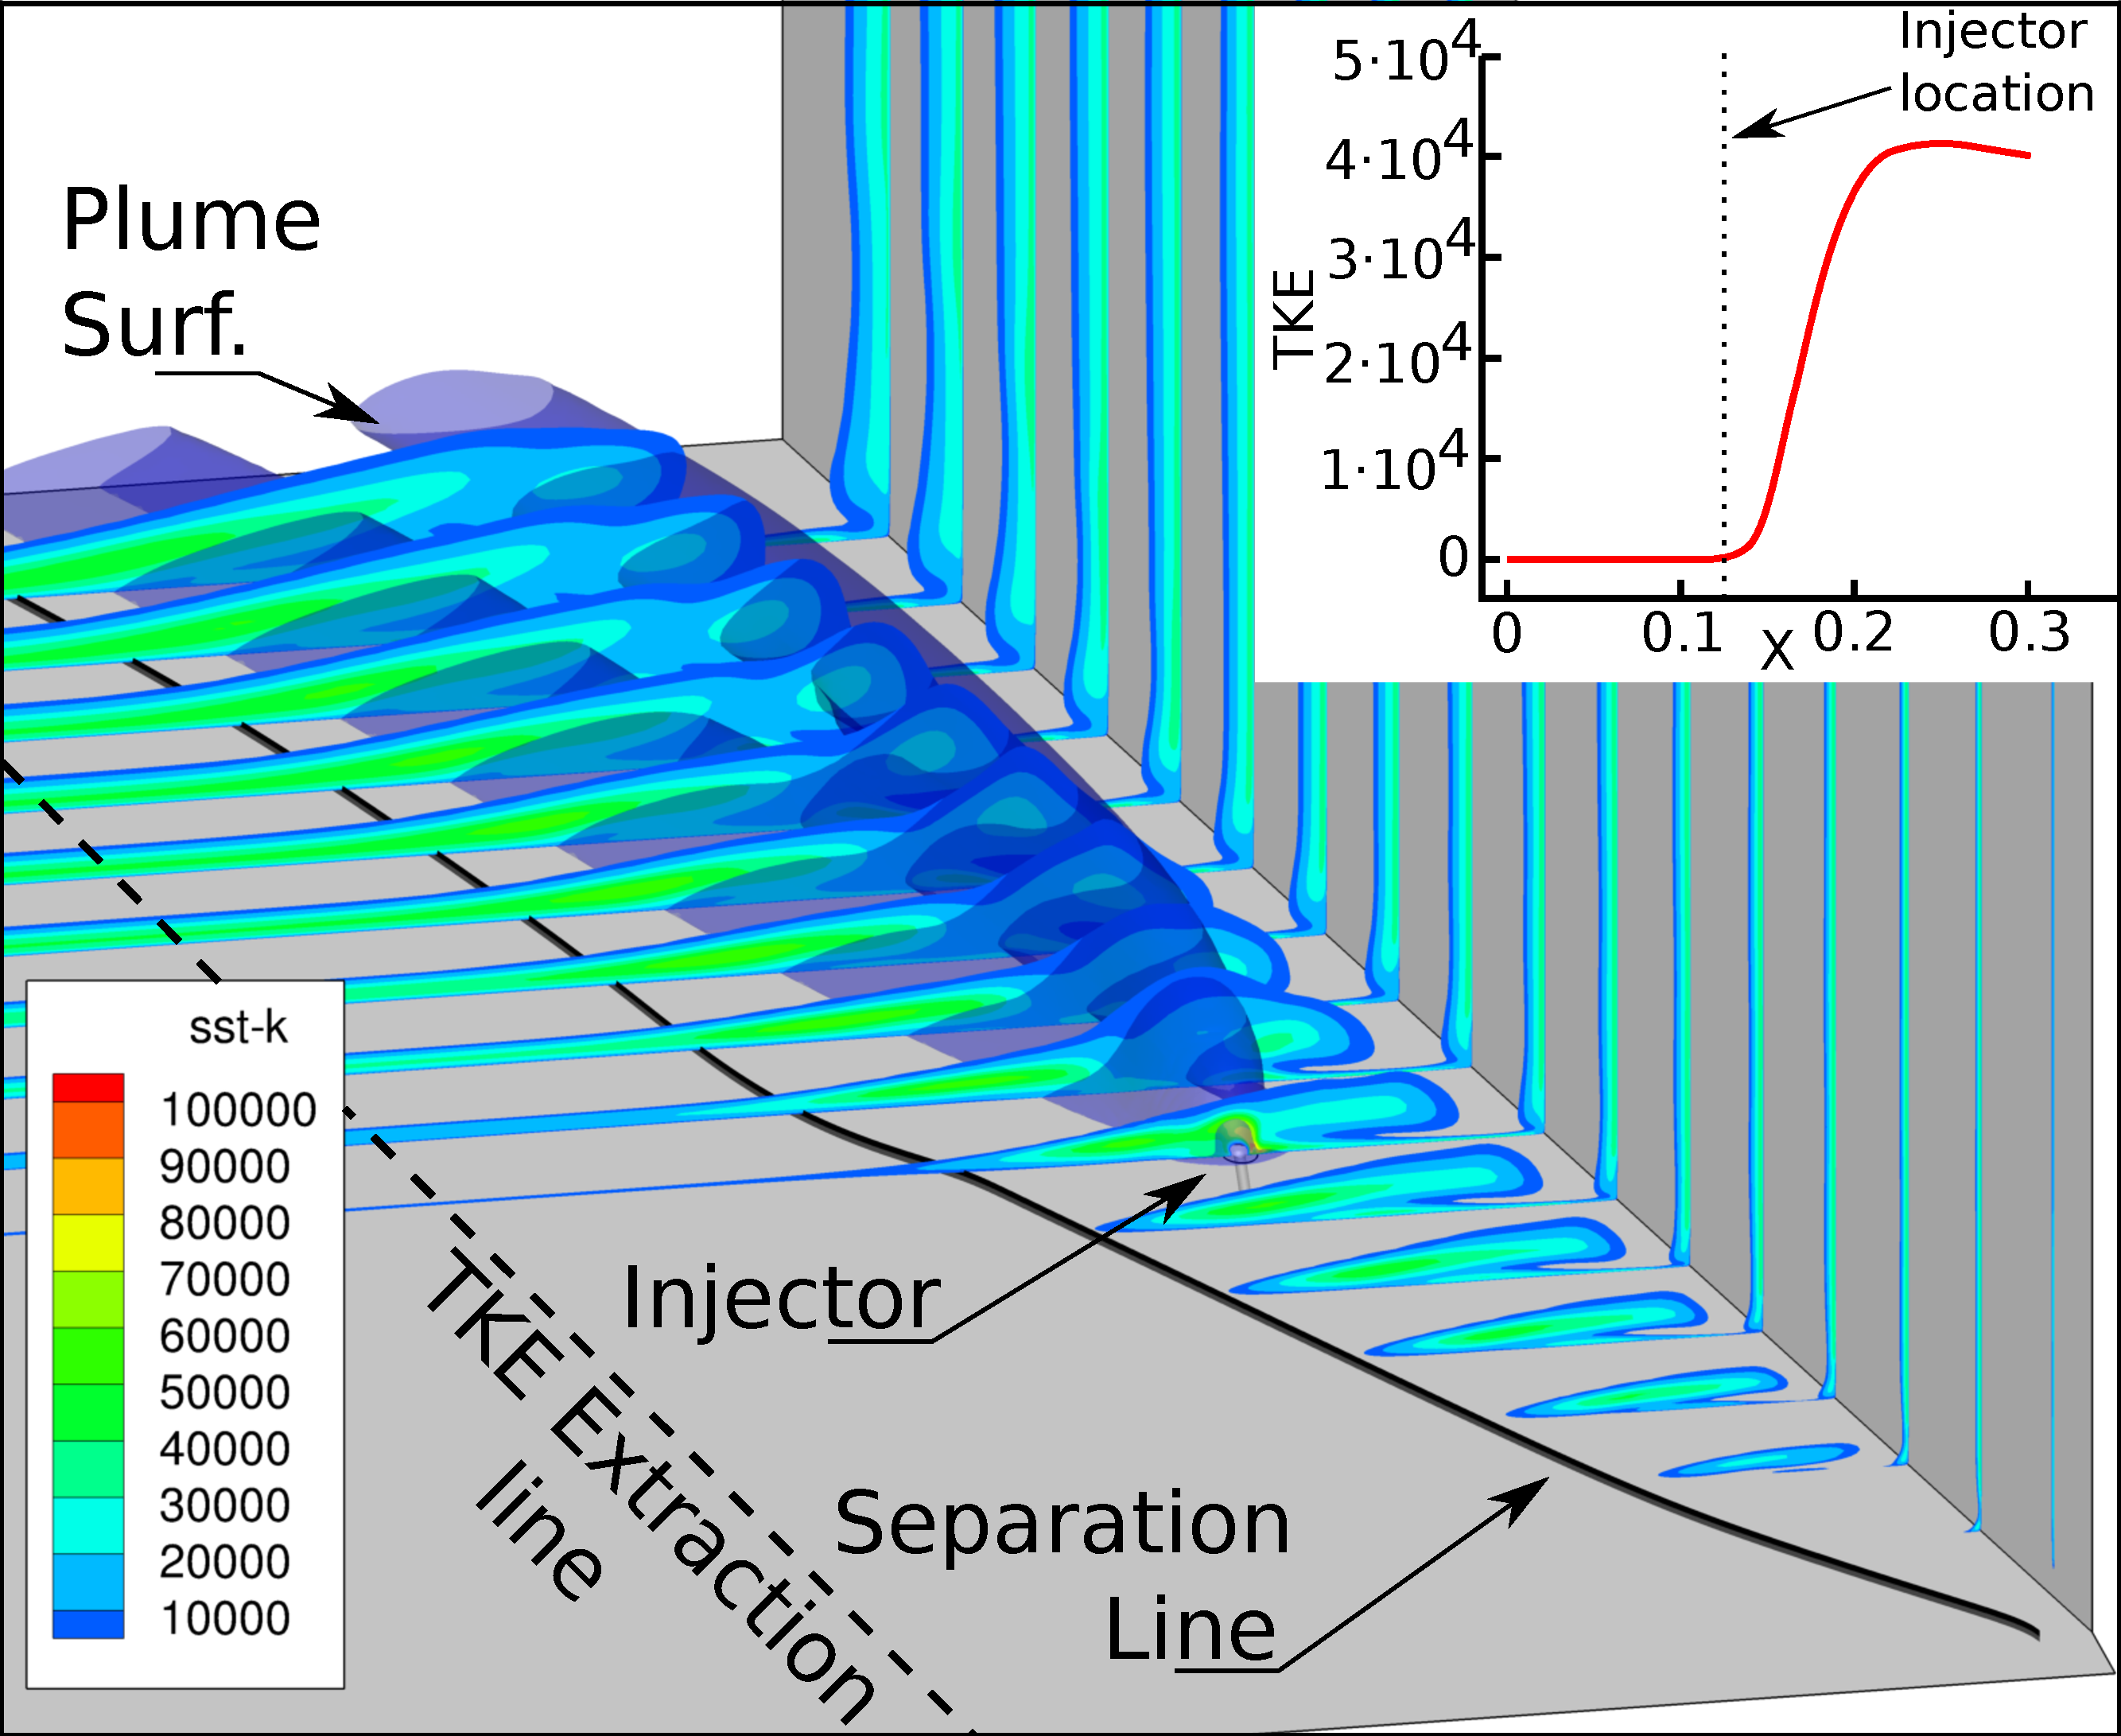
\includegraphics[trim = 0mm 0mm 0mm 0mm, clip, width=0.45\columnwidth]{Figures/TurbKinEnergySlices_csH2Stoich_LowP_LowF_HighInj_fmt_V2.pdf}
\label{fig:TurbKinEn_CFD_SliceLow}
}
\subfloat[Experimental and numerical heat flux on the undisturbed flat plate region.]{
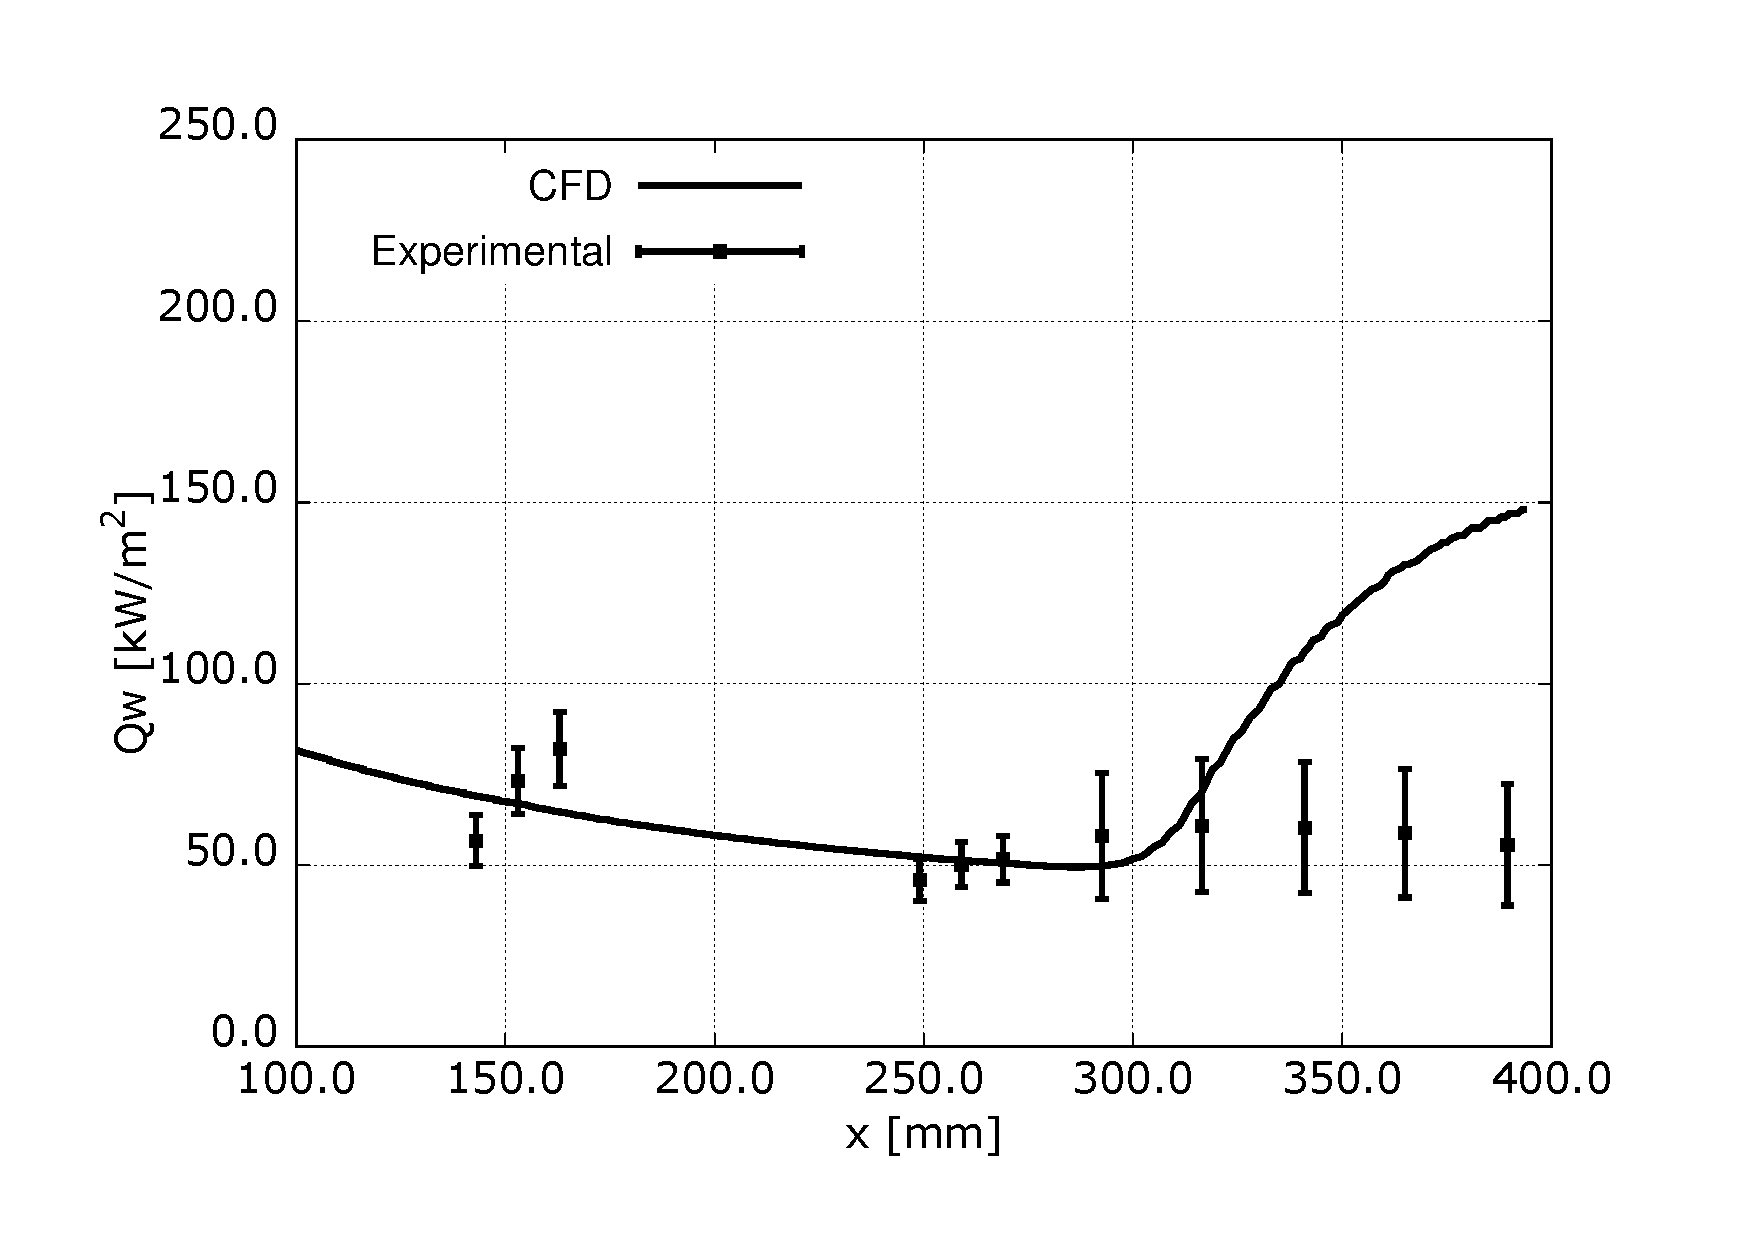
\includegraphics[trim = 0mm 6mm 25mm 18mm, clip, width=0.54\columnwidth]{Figures/GNUP_LP_CFD-EXP_Comparison.pdf}
\label{fig:Exp_Num_Q}
}
\caption{Boundary layer state comparison between the experimental and numerical cases}
\label{fig:Num_Exp_BLcompar}
\end{figure} 



%%%%%%%%%%%%%%%%%%%%%%%%%%%%%%%%%%%%%%%%%%%%%%%%%%%%%%%%%%%%%%%%%%%%%%%%%%%%%
\section{Results}

The experimental and numerical results for the six tests cases outlined in Table~\ref{tab:T4_Test_Cases} is presented here.
The no injection case will be presented first to outline the baseline interaction followed by the vortex-injection cases and how these different scenarios influenced the flowfield.

%%%%%%%%%%%%%%%%%%%%
\subsection{Unfueled vortex}

Two baseline cases using the UF and LF positions with no injection were performed to identify the effect that the induced vortex had on the TFHGs in the experiment and to show how well the numerical methodology was able to accurately simulate the flowfield.
Shown in Fig.~\ref{fig:HeatFluxVortex_Lines}, the numerical simulation heat-flux slices presented are aligned with the TFHG mounts in the experimental model to allow for a more accurate comparison.


%LP_NoI_UF
\begin{figure}[!h]
\center
%\begin{adjustbox}{max width=1.1\columnwidth,center}
\subfloat[Upper fin position.]{
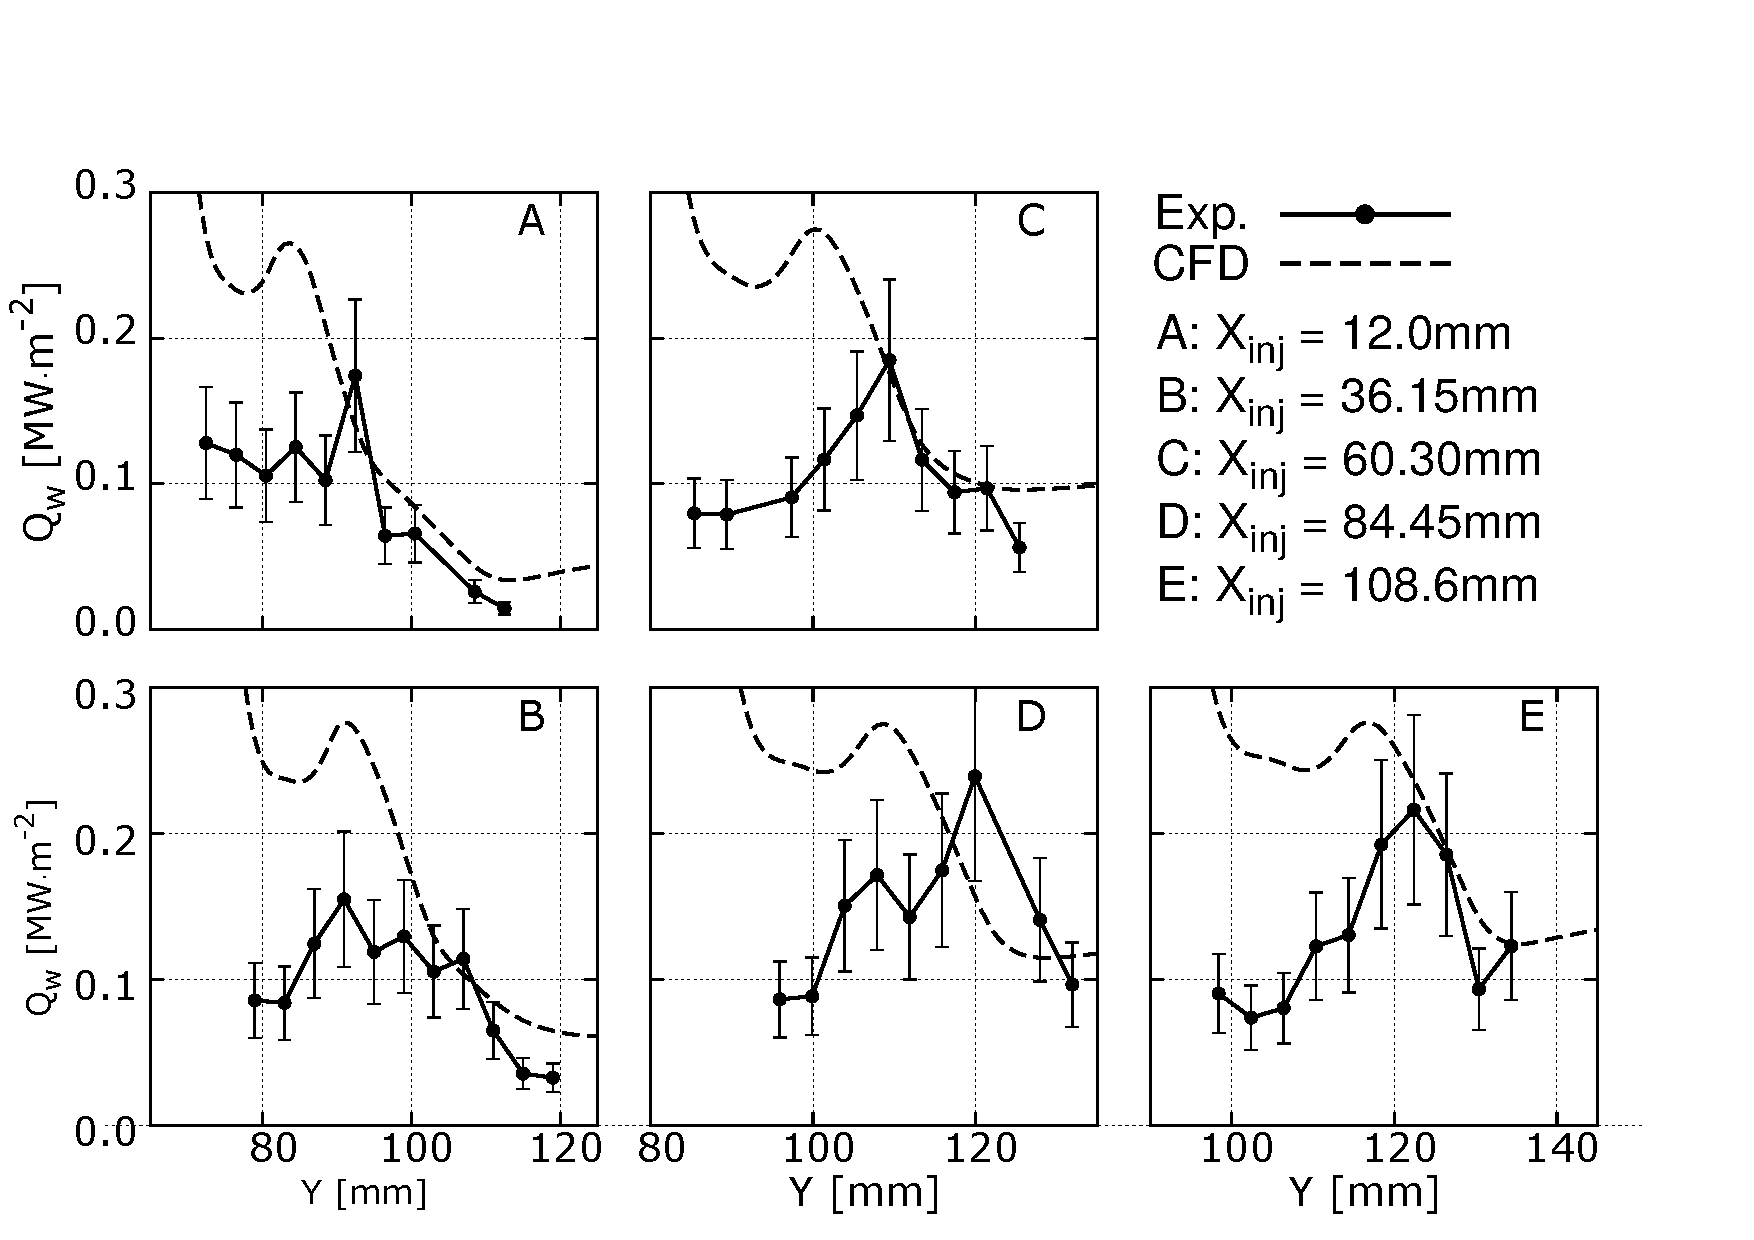
\includegraphics[trim = 0mm 3mm 25mm 25mm, clip, width=0.60\columnwidth,valign=t,fbox]{Figures/Data/LP_NoI_UF/GNUP_CFD_GaugesLines_Multi.pdf}
\label{fig:LP-NI-UF_LinesPlots}
}
%
\\
\subfloat[Lower fin position.]{
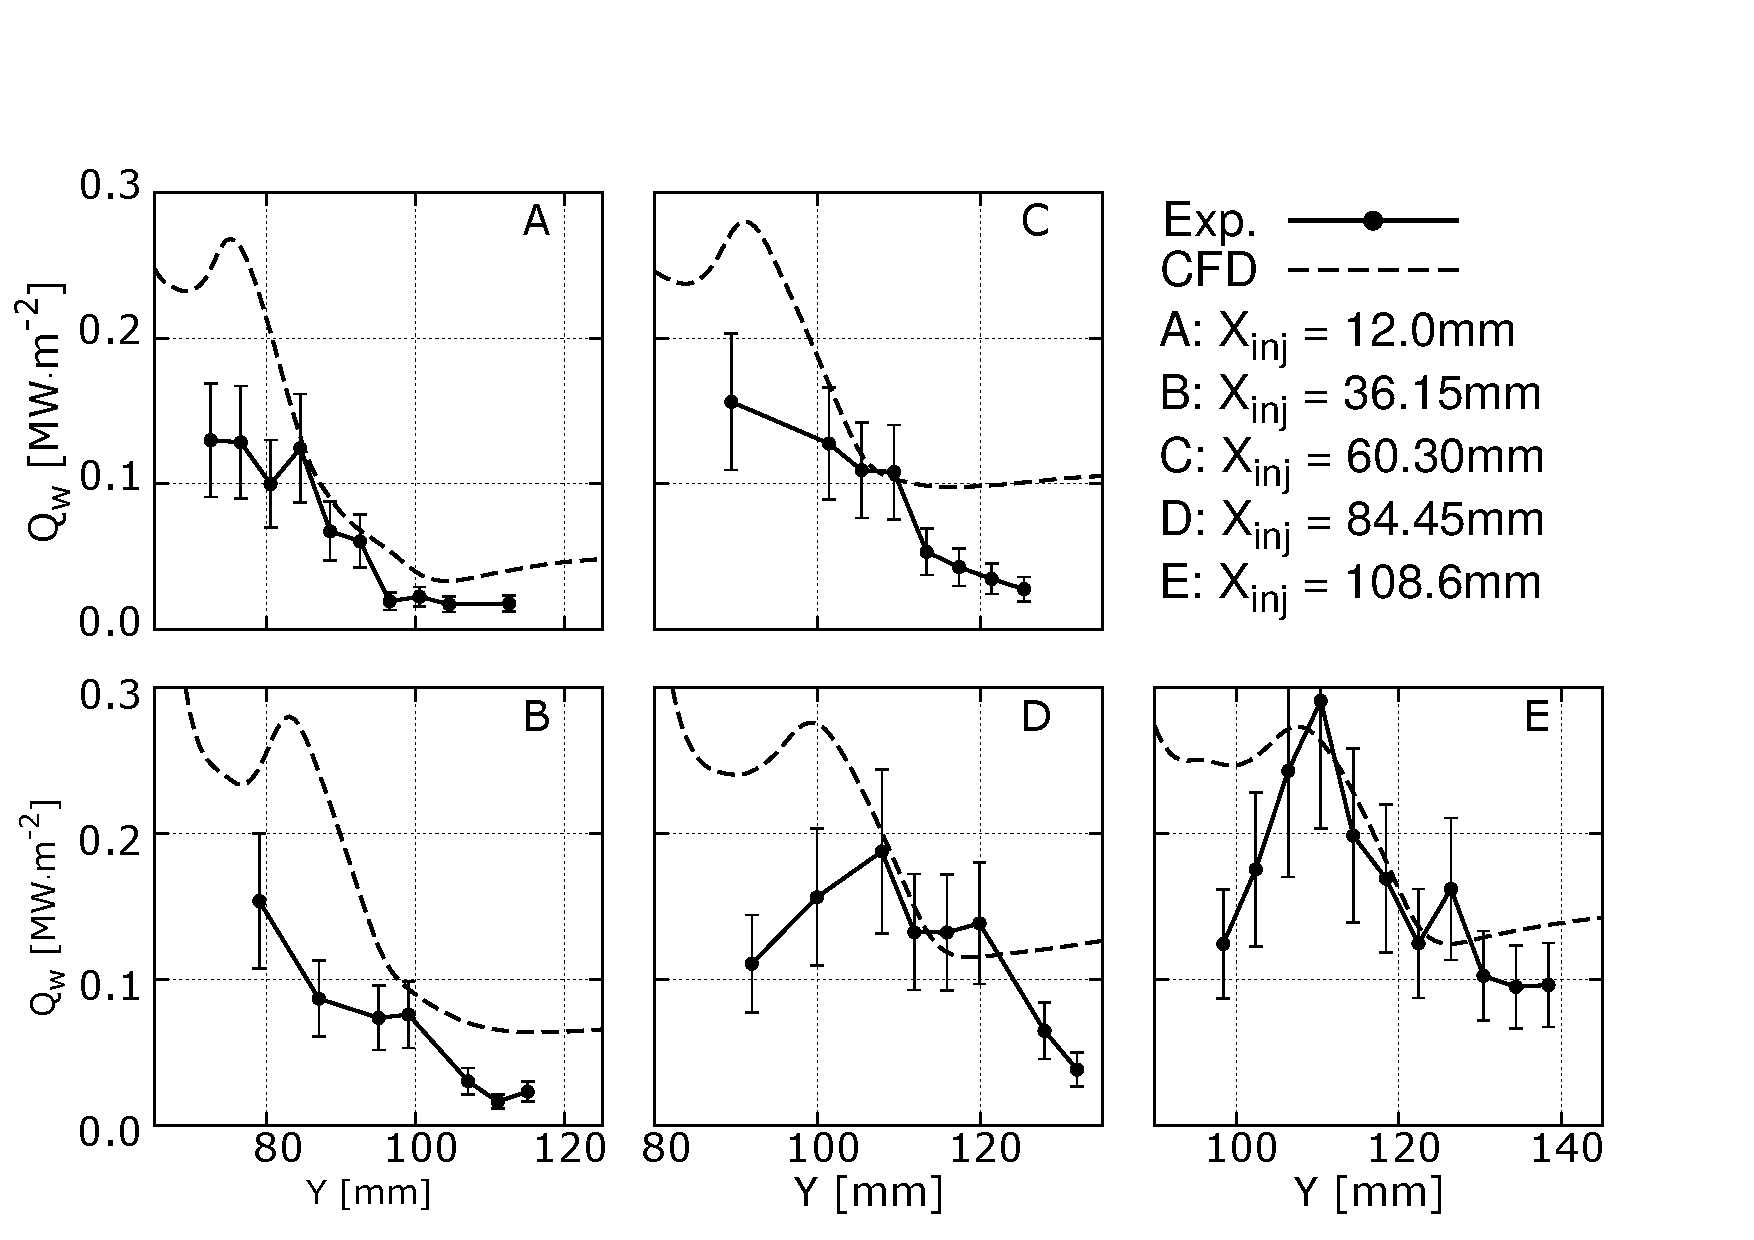
\includegraphics[trim = 0mm 3mm 25mm 25mm, clip, width=0.60\columnwidth,valign=t,fbox]{Figures/Data/LP_NoI_LF/GNUP_CFD_GaugesLines_Multi.pdf}
\label{fig:LP-NI-LF_LinesPlots}
}
%\end{adjustbox}
\caption{Numerical and experimental data on gauges lines A to E, at $X_{inj}$ axial distance from the injector. Unfuelled vortex cases.}
\label{fig:HeatFluxVortex_Lines}
\end{figure} 


Subsets Fig.~\ref{fig:LP-NI-UF_LinesPlots} and Fig.~\ref{fig:LP-NI-LF_LinesPlots} are separated out into the different upper and lower fin positions respectively.
For both cases, the further you traverse in the spanwise direction away from the oblique shock, the better the agreement.
However, in the region closest to the fin (defined as low Y values), the heat flux is overestimated in the numerical results.
This overestimation in the numerical data is consistent across the entire comparable domain, and it is visibly more prominent in the UF case.
This fact is induced by the closer proximity of the fin to the TFHG in the UF case, placing more gauges inside the region of overpredicted heat transfer. 


\begin{figure}[!h]
\center
\begin{adjustbox}{max width=1.1\columnwidth,center}
\subfloat[Experimental heat flux map. Solid dots are active gauges. Hollow dots are discarded gauges.]{
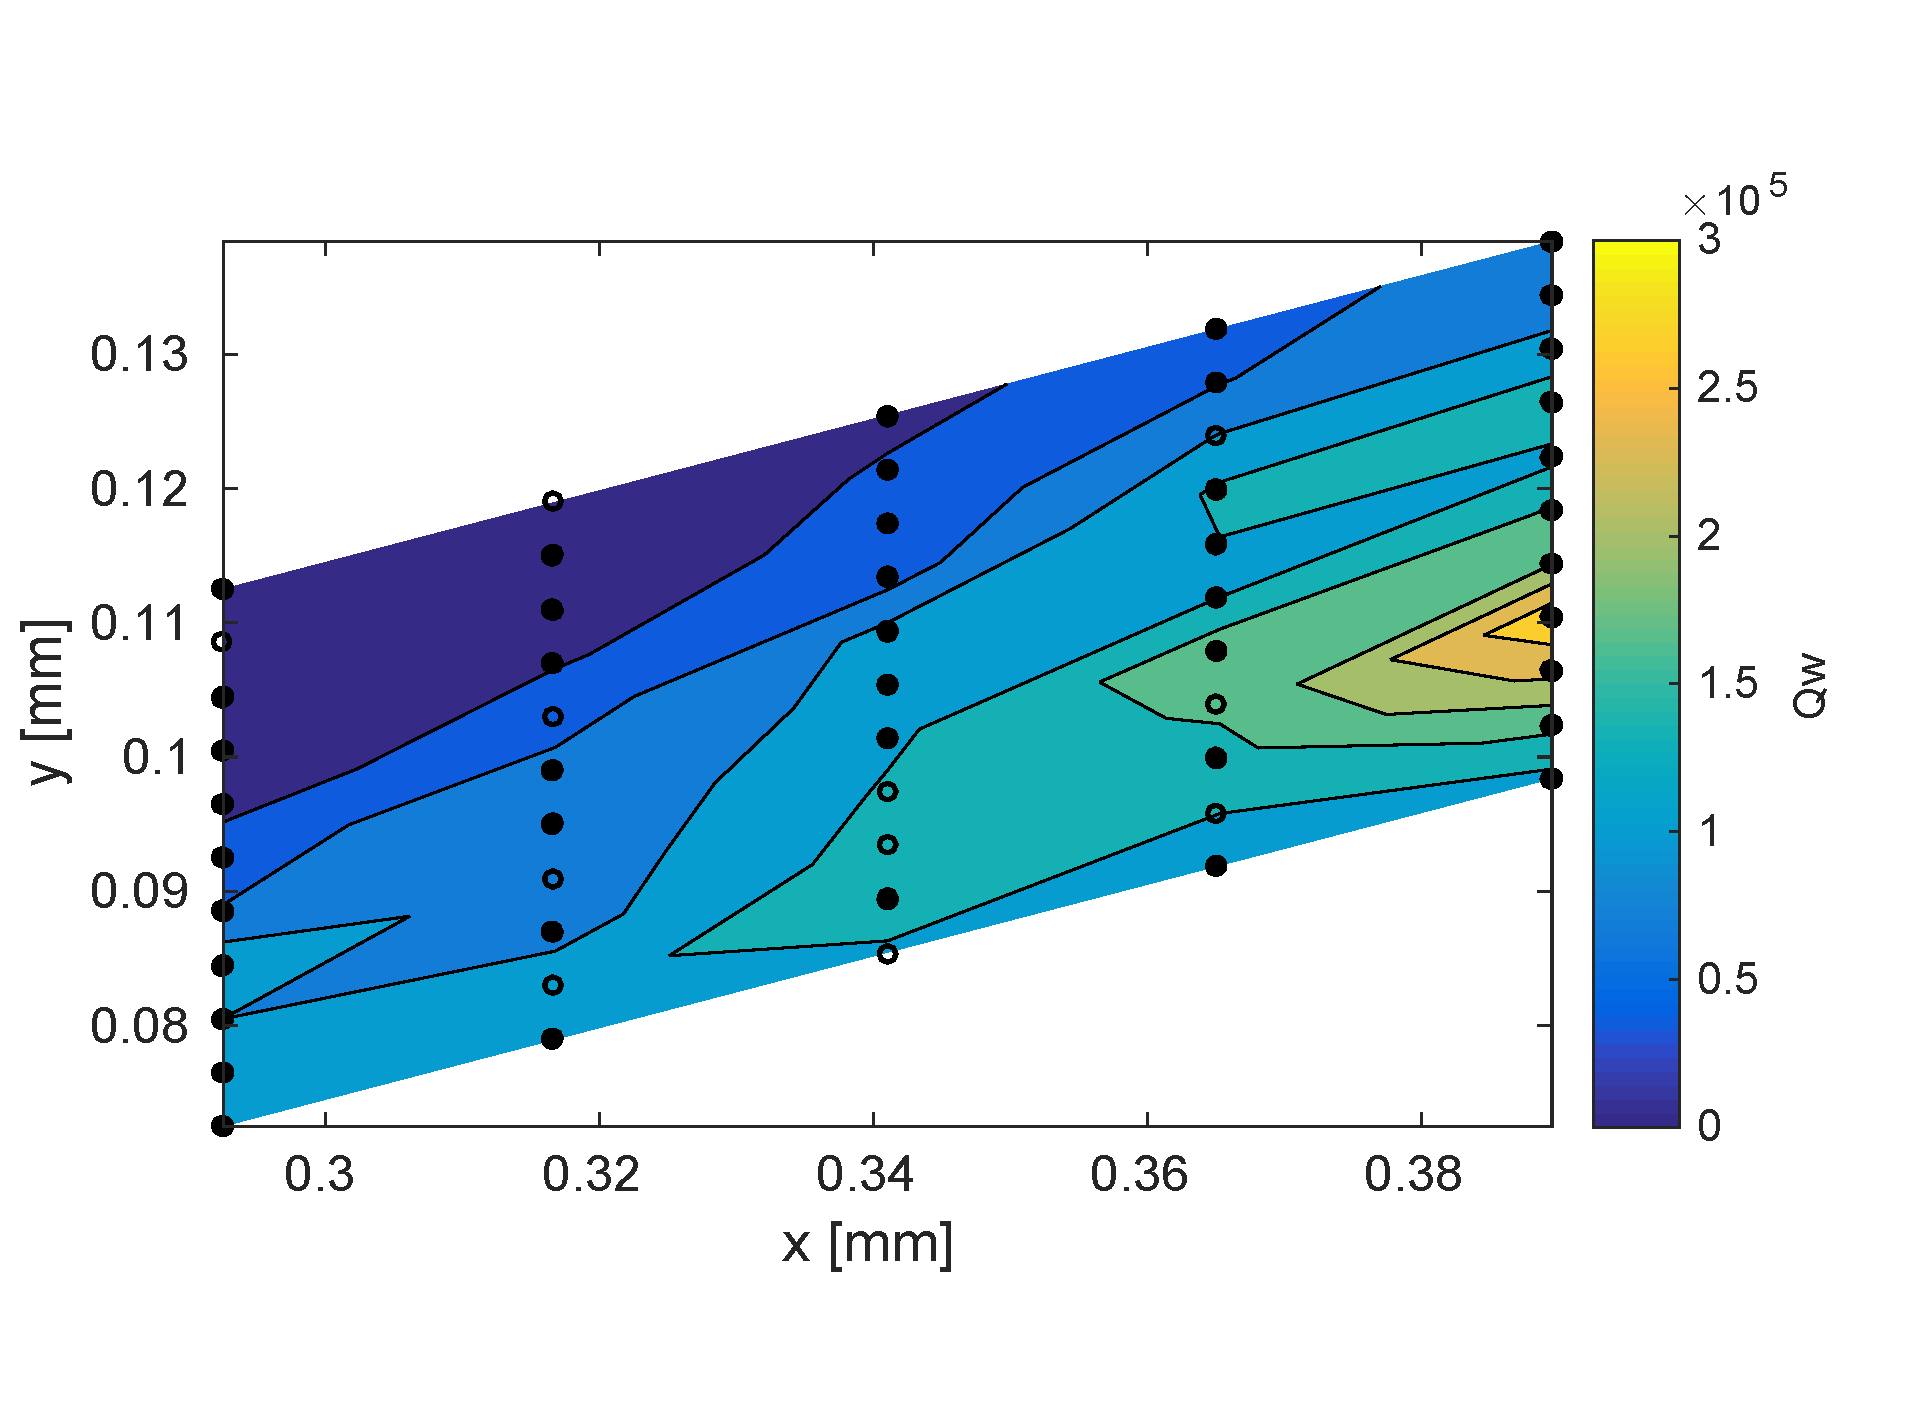
\includegraphics[trim = 0mm 12mm 5mm 12mm, clip, width=0.50\columnwidth,valign=t]{Figures/Data/LP_NoI_LF/Post-processed_GaugesQMap.png}
\label{fig:NI-LF_QwMap}
}
%
\subfloat[Numerical heat flux map. Dotted line indicates experimental acquisition area. Dashed red line indicates separation line. Solid red line indicates location of inviscid fin shock.]{
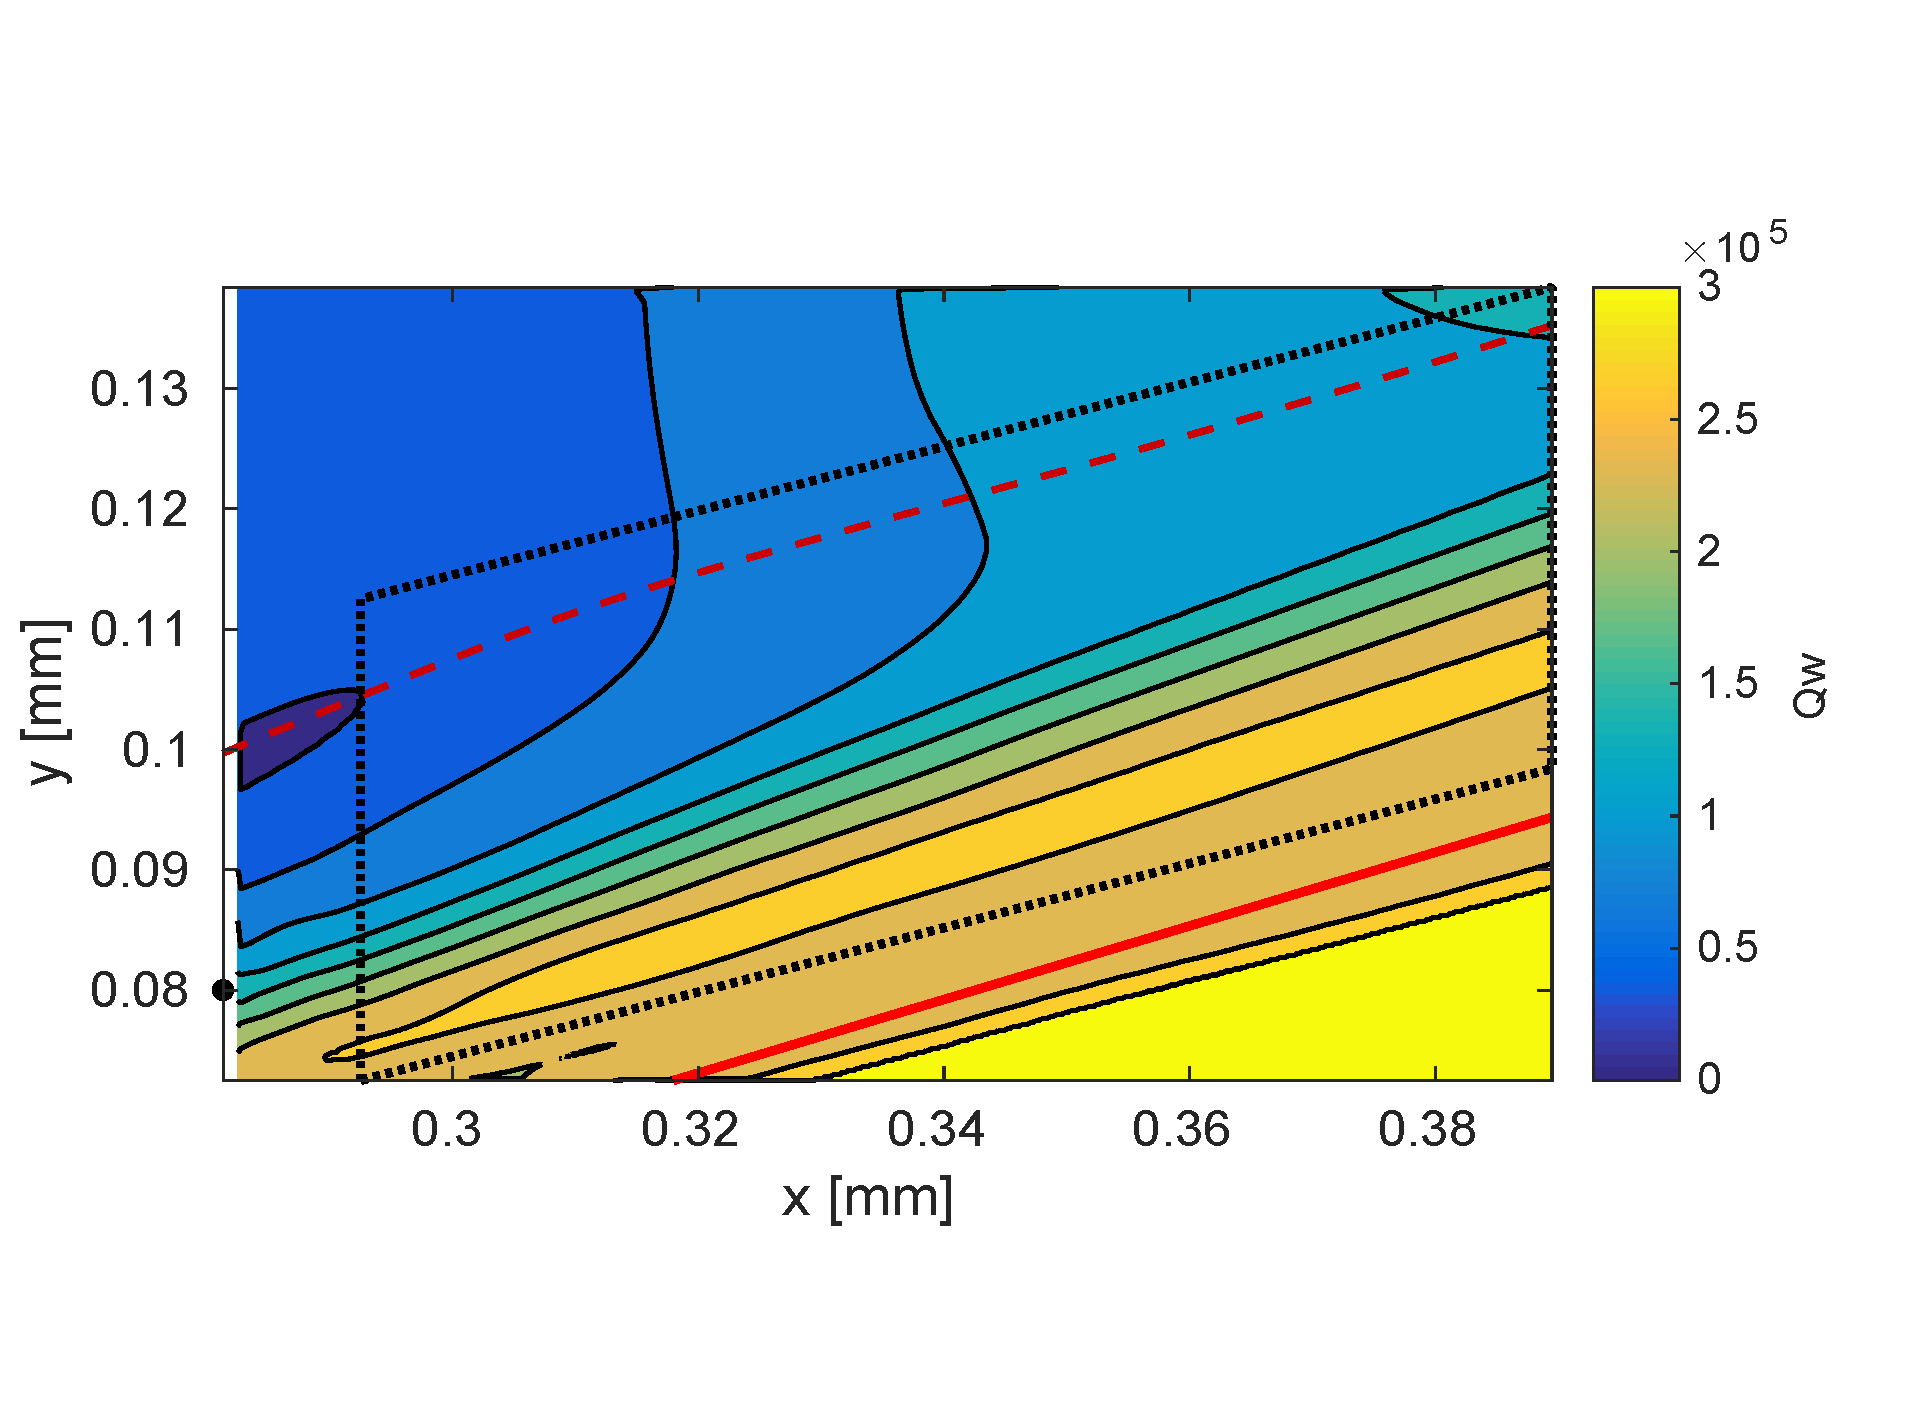
\includegraphics[trim = 0mm 15mm 5mm 17mm, clip, width=0.55\columnwidth,valign=t]{Figures/Data/LP_NoI_LF/Post-processed_CFDB.png}
\label{fig:NI-LF_cfdQwMap}
}
\end{adjustbox}
\caption{Recontructed heat transfer map. Comparison of heat flux from experiments and CFD. NI-LF (Case 2 in Table~\ref{tab:T4_Test_Cases}).}
\label{fig:HeatFluxNILF}
\end{figure} 



Figure~\ref{fig:HeatFluxNILF} presents an extrapolated mapped version of the experimental data along with the equivalent numerical comparison for the LF case.
In this position, the fin is placed further from the TFHGs and therefore, a smaller part of the numerically overpredicted heat-flux lays within the measurement region.
Also, shown on the figure is the vortex flowfield separation and reattachment lines.
The reattachment takes place behind the fin shock, driving hot and dense shock compressed gas towards the flat plate, as labeled in Fig.~\ref{fig:Alvi_Sketch} as 'jet'.
This reattachment takes place in the region close to the fin where the numerical simulations over predict the heat flux.
Assuming that the viscous shock process is accurately modeled, the overestimation of the heat flux is predicted to be caused by an overestimation of the turbulence intensity in the region.
This can be observed in Fig.~\ref{fig:SSTk_Q_Combi} which shows line A from the UF case (Fig.~\ref{fig:LP-NI-UF_LinesPlots}) combined with the TKE from the same axial location.
The point where the numerical estimation begins to diverge from the experimental results, as shown on the figure, is coincident with an increase in the level of TKE adjacent to the model surface.
The blown up image in Fig.~\ref{fig:SSTk_Q_Combi} shows a better representation of this elevated TKE region.
What this region suggests is that the turbulence model is overpredicting the level of turbulence, and thus the heat flux into the wall.


%
\begin{figure}[!h]
\center
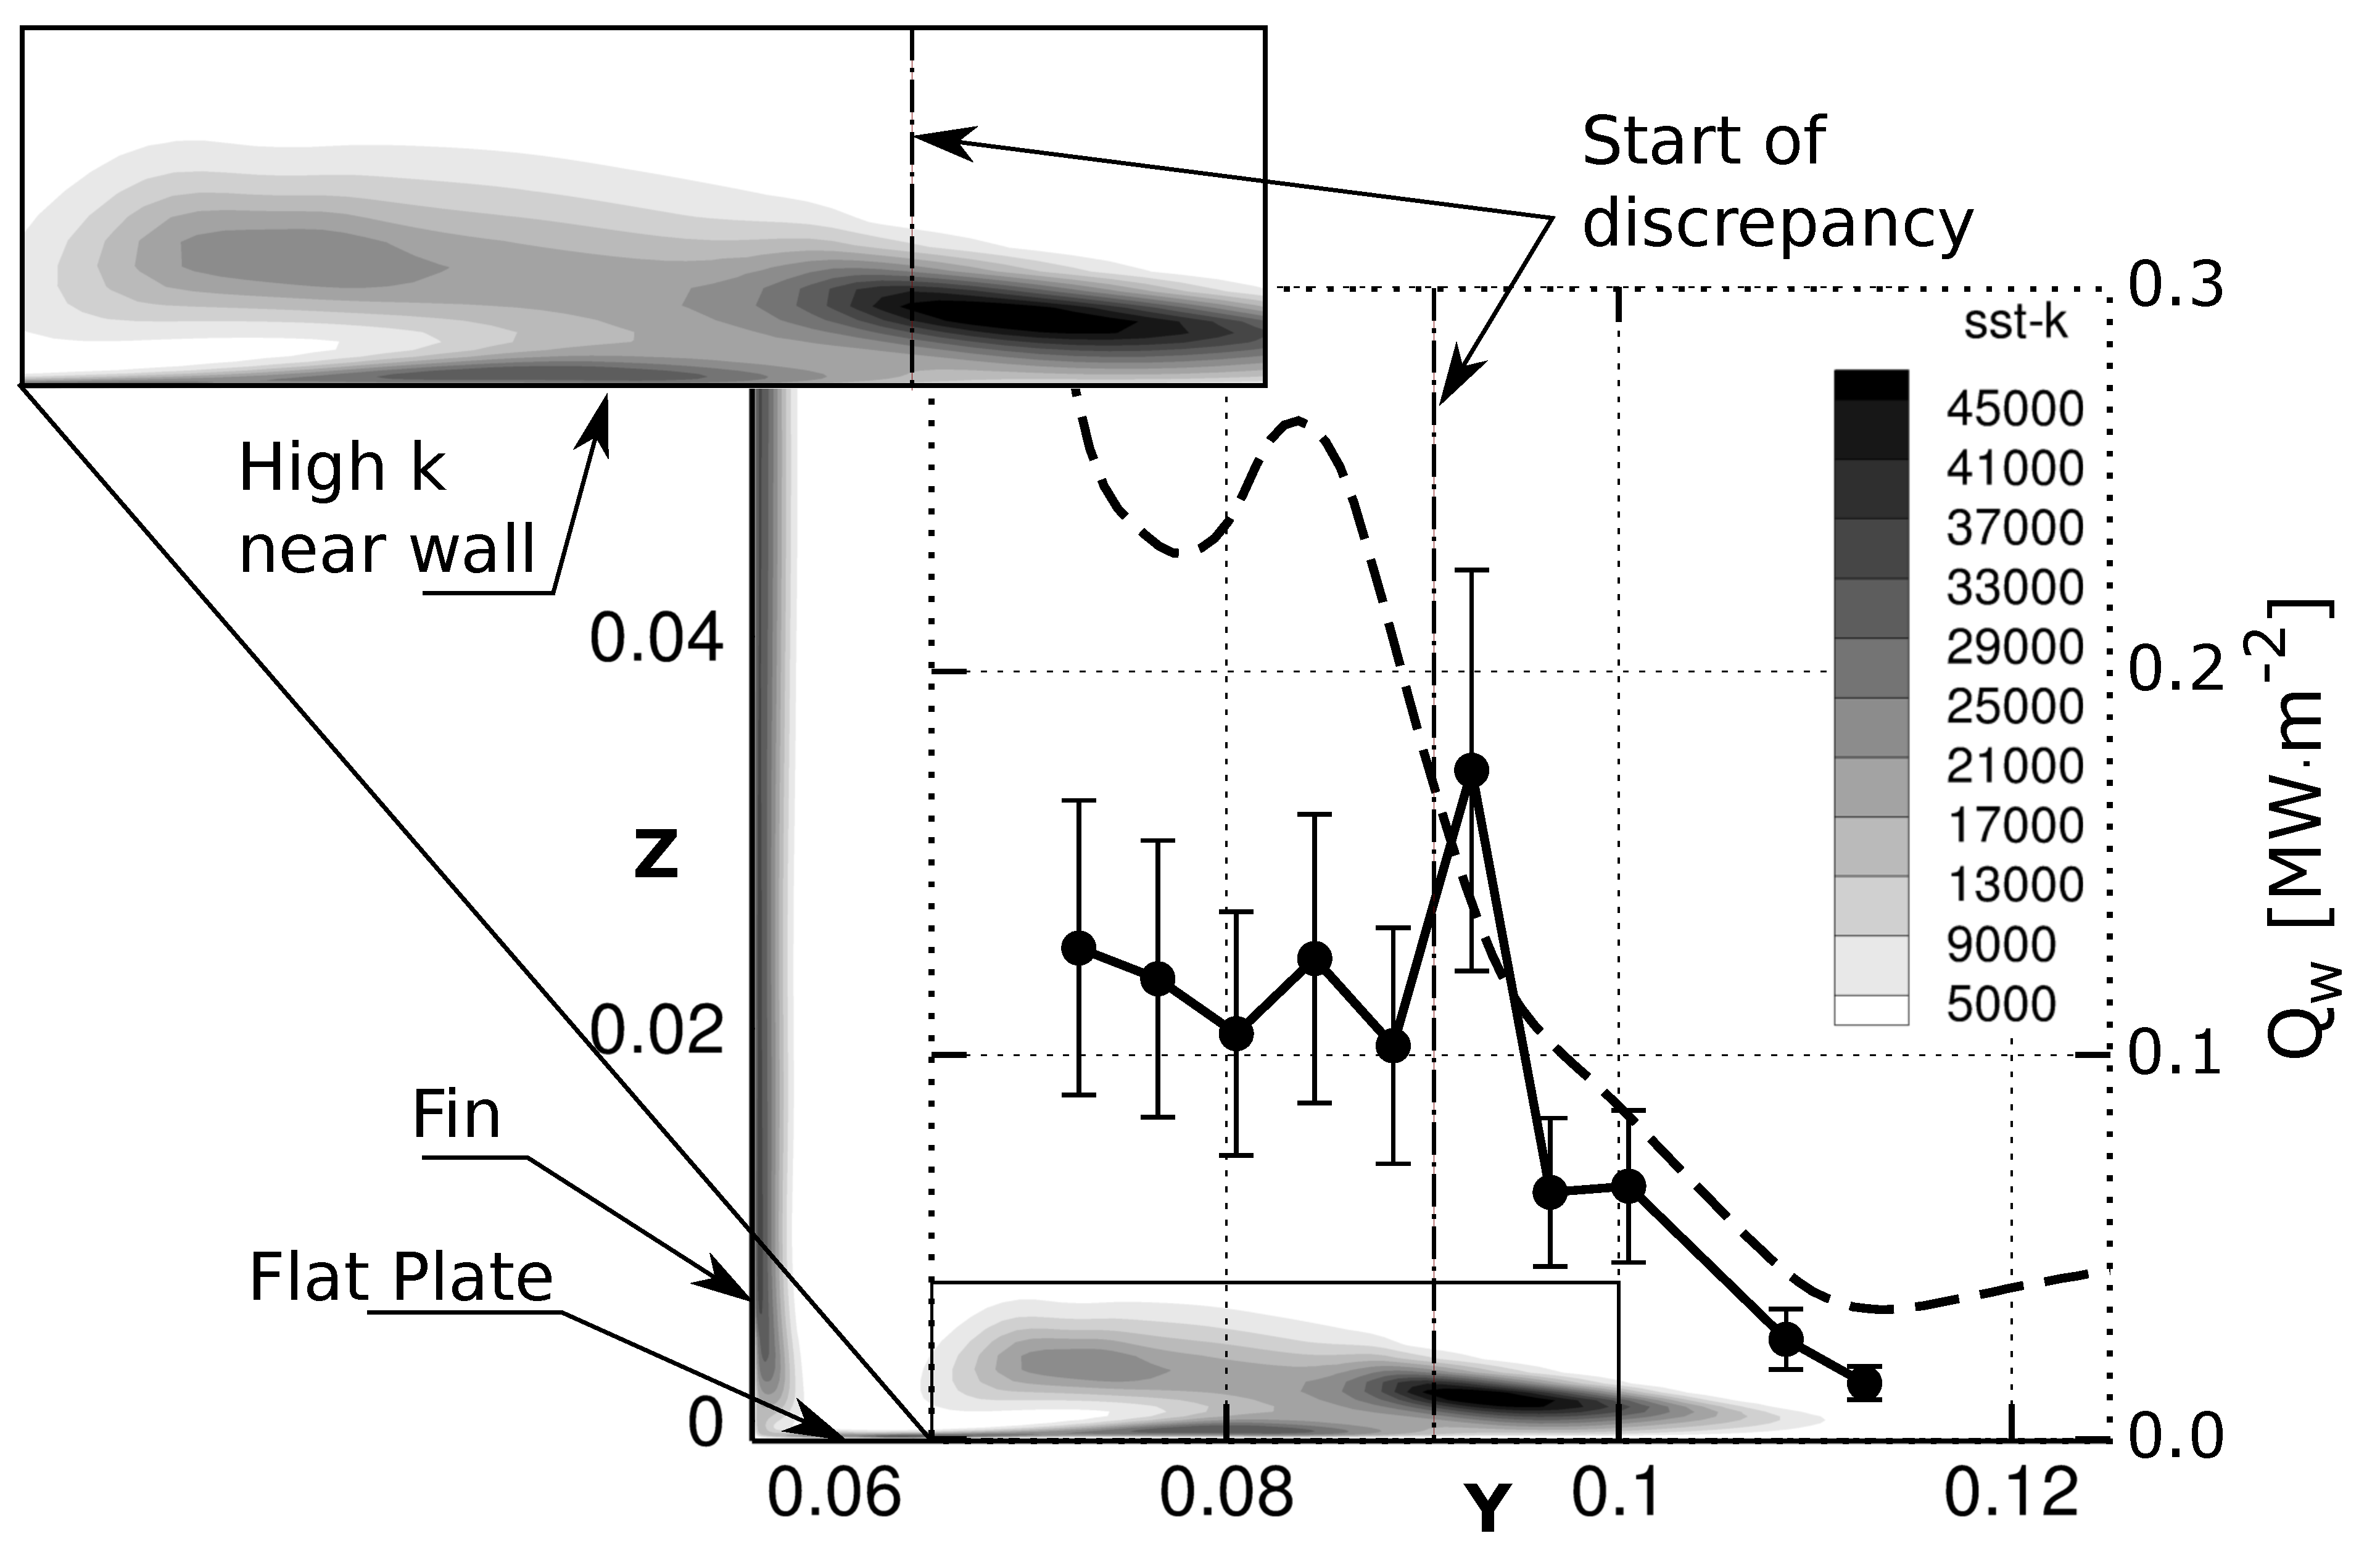
\includegraphics[width=0.70\columnwidth,valign=t]{Figures/SST-K_X137_LP_NI_UF_Q_and_SSTk_Combined.pdf}
\caption{Contours of turbulent kinetic energy combined with experimental and numerical heat flux at $X_{inj} = \SI{12}{\milli\meter}$.}
\label{fig:SSTk_Q_Combi}
\end{figure} 


This discrepancy created by the numerical solver being unable to accurately simulate the heat flux near the fin shock is a key aspect to take into account when comparing the numerical and experimental data from the fueled results. 
This region of overestimation will be referred to as the `numerical overestimation zone'.


%%%%%%%%%%%%%%%%%%%%
\subsection{Fuel vortex interaction}

The results obtained for the tests using the UF and LF positions in combination with the high and low injection pressures (cases 3-6 in Table~\ref{tab:T4_Test_Cases}) provide some initial data on the complex vortex-injection interaction flowfield.

%%%%%%%%%%%%%%%%%%%%
\subsubsection{Upper fin position, High injection pressure}

Both the experimental and numerical results for the high injection pressure UF case are presented in Fig.~\ref{fig:HeatFluxLPHIUF}.
Qualitatively, there is a good agreement between the numerical and experimental results far away from the fin wall.
The two curves have similar trends, and the heat flux peak induced by the injection bow shock was able to be simulated numerically.
However, the numerical heat flux values near the fin (low Y values) are again overestimated when compared to the experimental results.
This overestimation is caused by the presence of the `numerical overestimation zone' previously outlined for the NI case.

%
%LP_HI_UF
\begin{figure}[!h]
\center
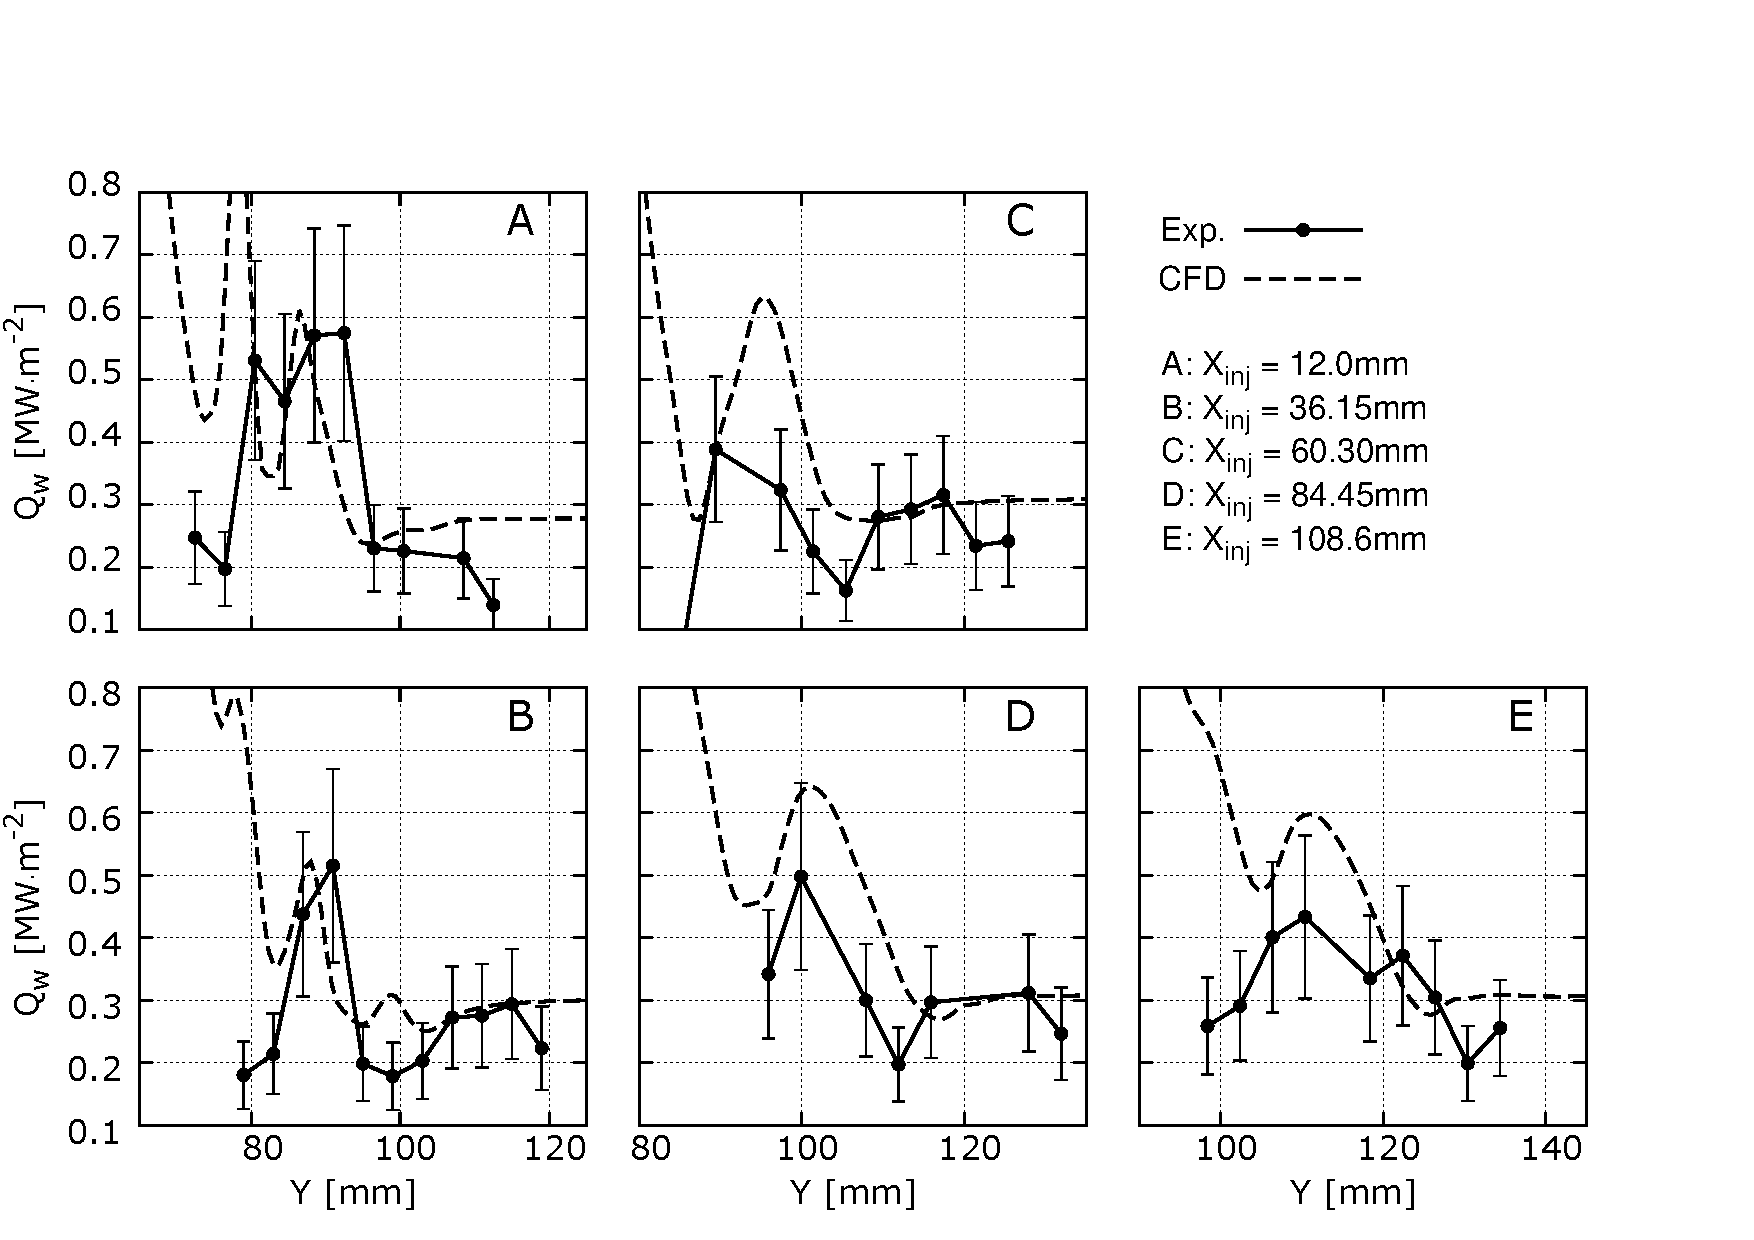
\includegraphics[trim = 0mm 3mm 25mm 25mm, clip, width=0.60\columnwidth,valign=t,fbox]{Figures/Data/LP_HI_UF/GNUP_CFD_GaugesLines_Multi.pdf}
\caption{Numerical and experimental heat transfer data. HI-UF (Case 1 in Table~\ref{tab:T4_Test_Cases})}
\label{fig:HeatFluxLPHIUF}
\end{figure} 


\begin{figure}[!h]
\center
\begin{adjustbox}{max width=1.1\columnwidth,center}
\subfloat[Experimental heat flux map. Solid dots are active gauges. Hollow dots are discarded gauges.]{
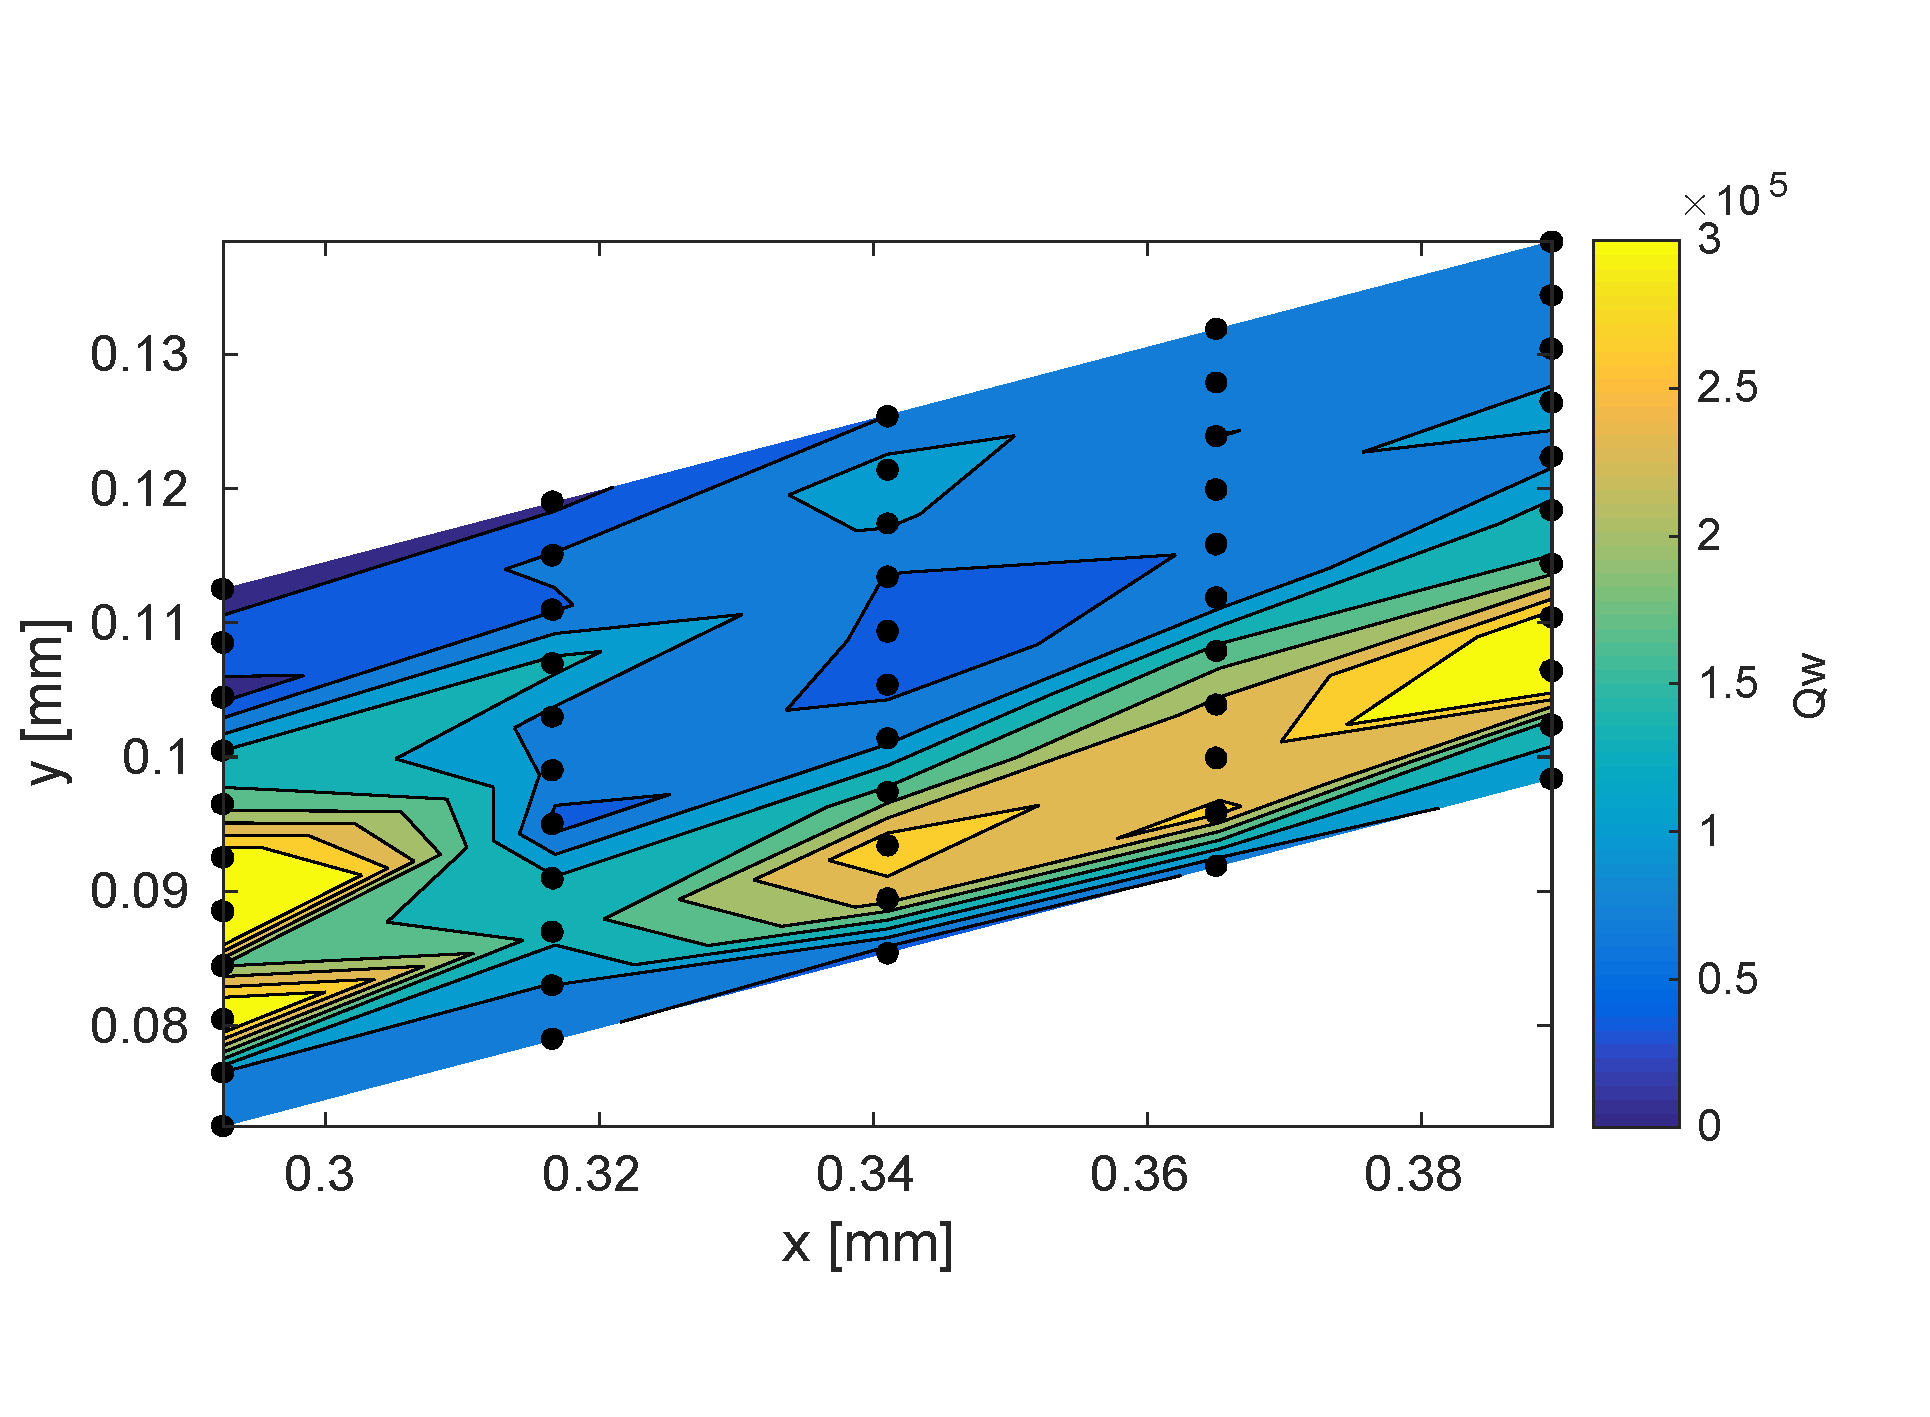
\includegraphics[trim = 0mm 12mm 5mm 12mm, clip, width=0.50\columnwidth,valign=t]{Figures/Data/LP_HI_UF/Post-processed_GaugesQMap.png}
\label{fig:LP-HI-UF_QwMap}
}
%
\subfloat[Numerical heat flux map. Dotted line indicates experimental acquisition area. Dashed red line indicates separation line. Solid red line indicates location of inviscid fin shock.]{
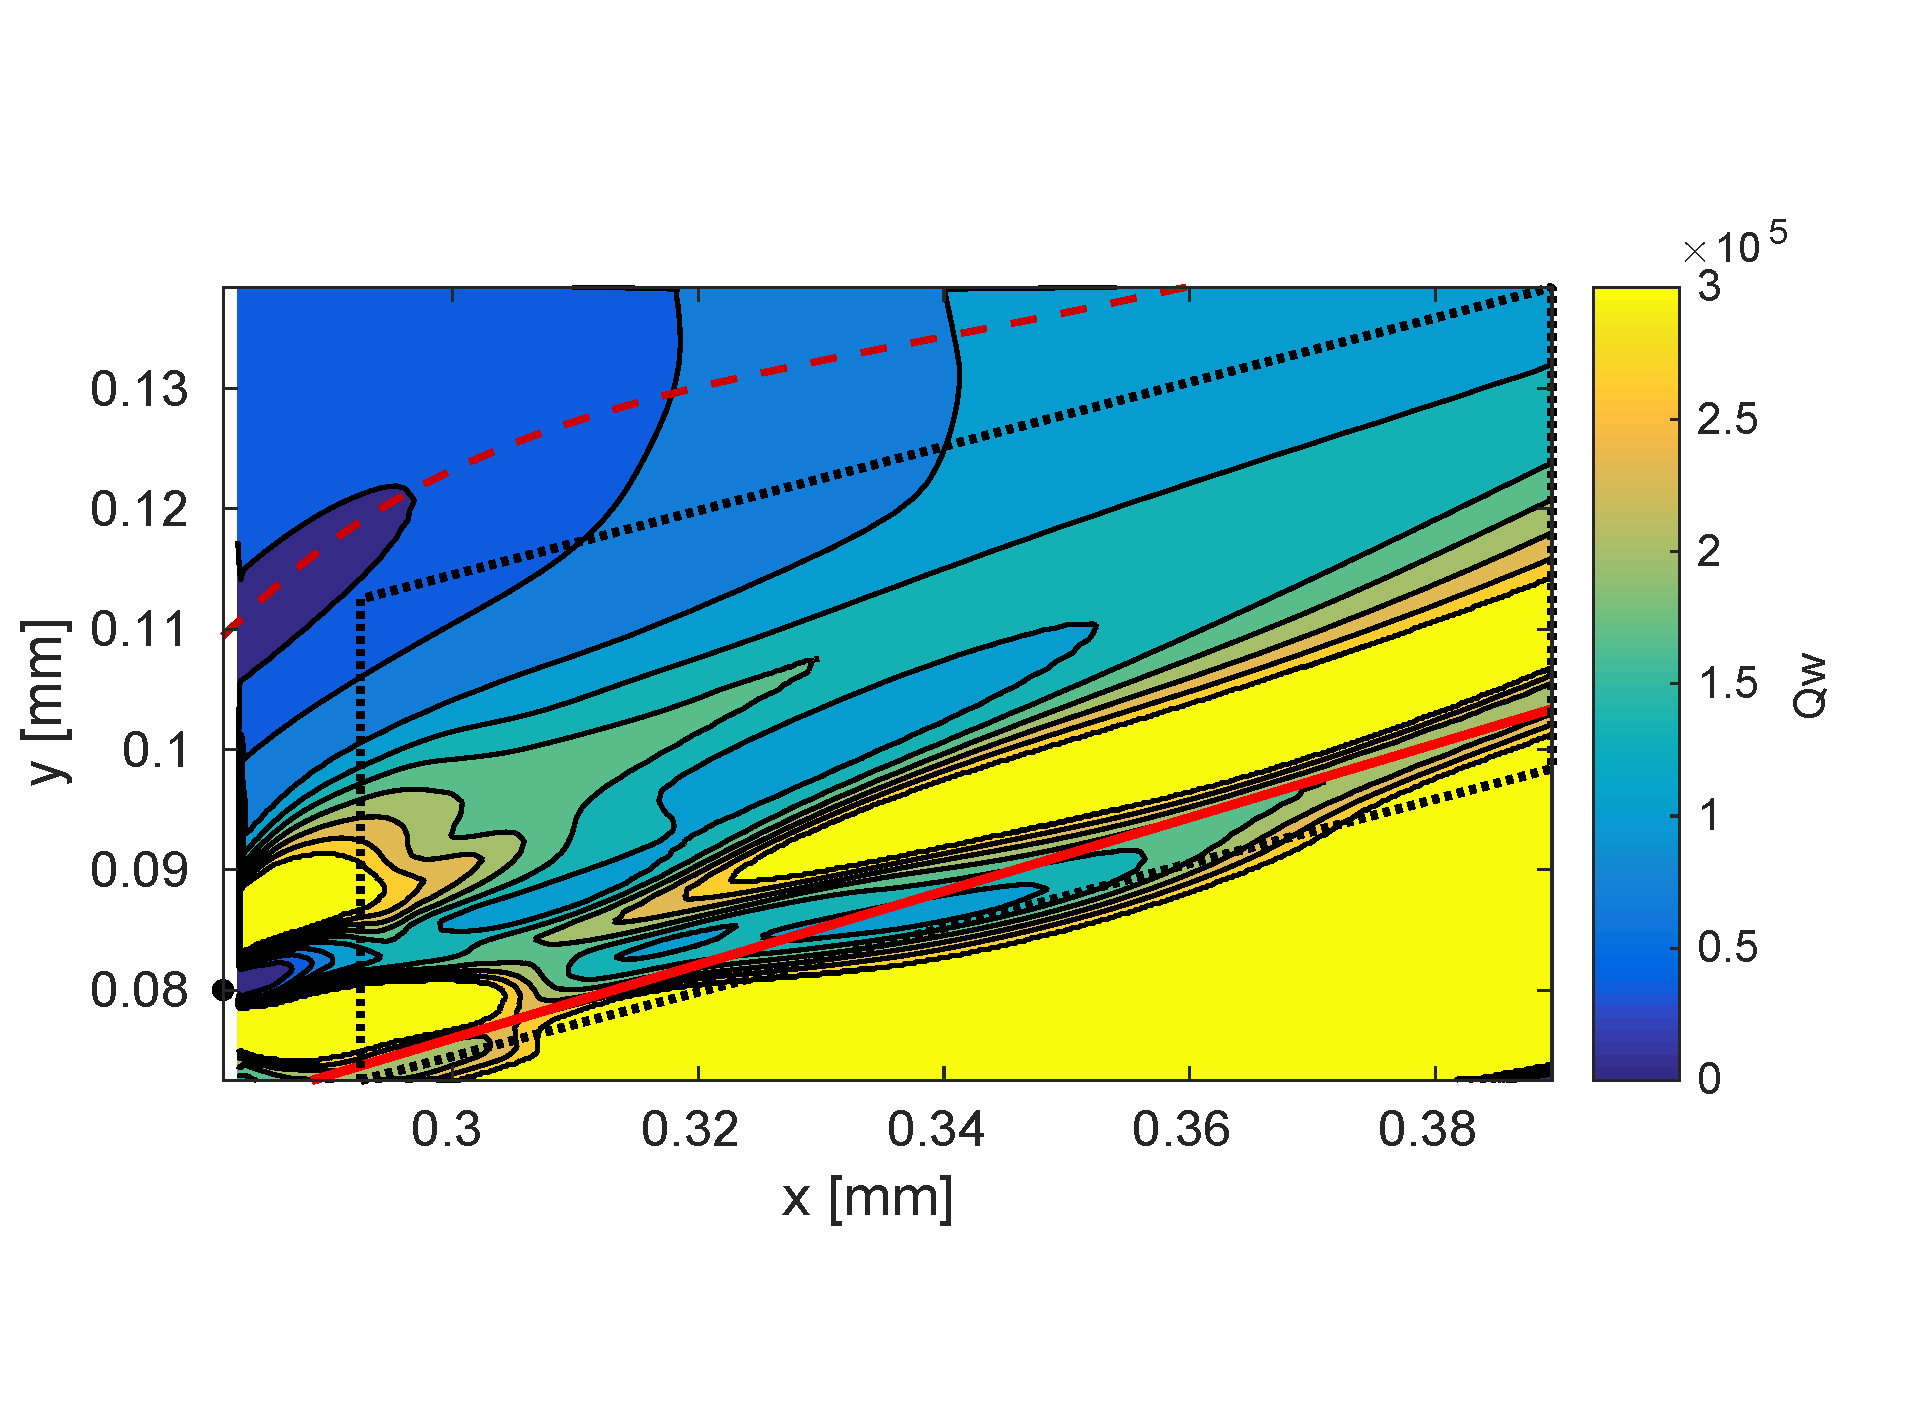
\includegraphics[trim = 0mm 15mm 5mm 17mm, clip, width=0.55\columnwidth,valign=t]{Figures/Data/LP_HI_UF/Post-processed_CFDB.png}
\label{fig:LP-HI-UF_cfdQwMap}
}
\end{adjustbox}
\caption{Recontructed heat transfer map. Comparison of heat flux from experiments and CFD. HI-UF (Case 3 in Table~\ref{tab:T4_Test_Cases})}
\label{fig:HeatFluxMap}
\end{figure} 


%%%%%%%%%%%%%%%%%%%%
\subsubsection{Flowfield description from numerical data}

The numerical solution presents an interesting heat flux distribution on the flat plate consisting of a strip of elevated levels running approximately longitudinally down the center of the vortex.
This regions extends from shortly downstream of the injection bow shock up to the end of the experimental measurements.
This feature is difficult to visualize in Fig.~\ref{fig:HeatFluxLPHIUF}, but is apparent in the heat flux maps shown in Fig.~\ref{fig:HeatFluxMap}.
This elevated strip is coupled with a neighboring decreased heat flux strip, both highlighted in Fig.~\ref{fig:Exper_Flowf}.
Where Fig.~\ref{fig:Exper_Flowf} presents the three-dimensional numerical data showing the vortex-injection interaction. 


Figure~\ref{fig:Exper_Flowf}a displays the evolution of the flow upstream of the injector to the far-field downstream on the plate.
The fuel plume begins with a nearly hemispheric shape and evolves to a highly elongated profile. 
Far downstream, the fuel plume splits into two regions, one located within the vortex recirculation region, and the other adjacent to the flat plate wall.
This region of interest is presented in more detail in Fig.~\ref{fig:Exper_Flowf}b.
In this figure, the streak lines on the model surface show the elevated and decreased heat flux strips are coincident with the separation and reattachment of the flow.
These two stream lines (separation and reattachment) are linked to a counter rotating vortex shown in in Fig.~\ref{fig:Exper_Flowf}c, marked as `C.R. vortex'.


% KDB: You need axes on this or flow direction or something, it's hard to figure out what the reattchement pciture is tryign to show or where the vortex cross section ceomss from. I like this figure but just needs that last little bit. 
\begin{figure}[!h]
\center
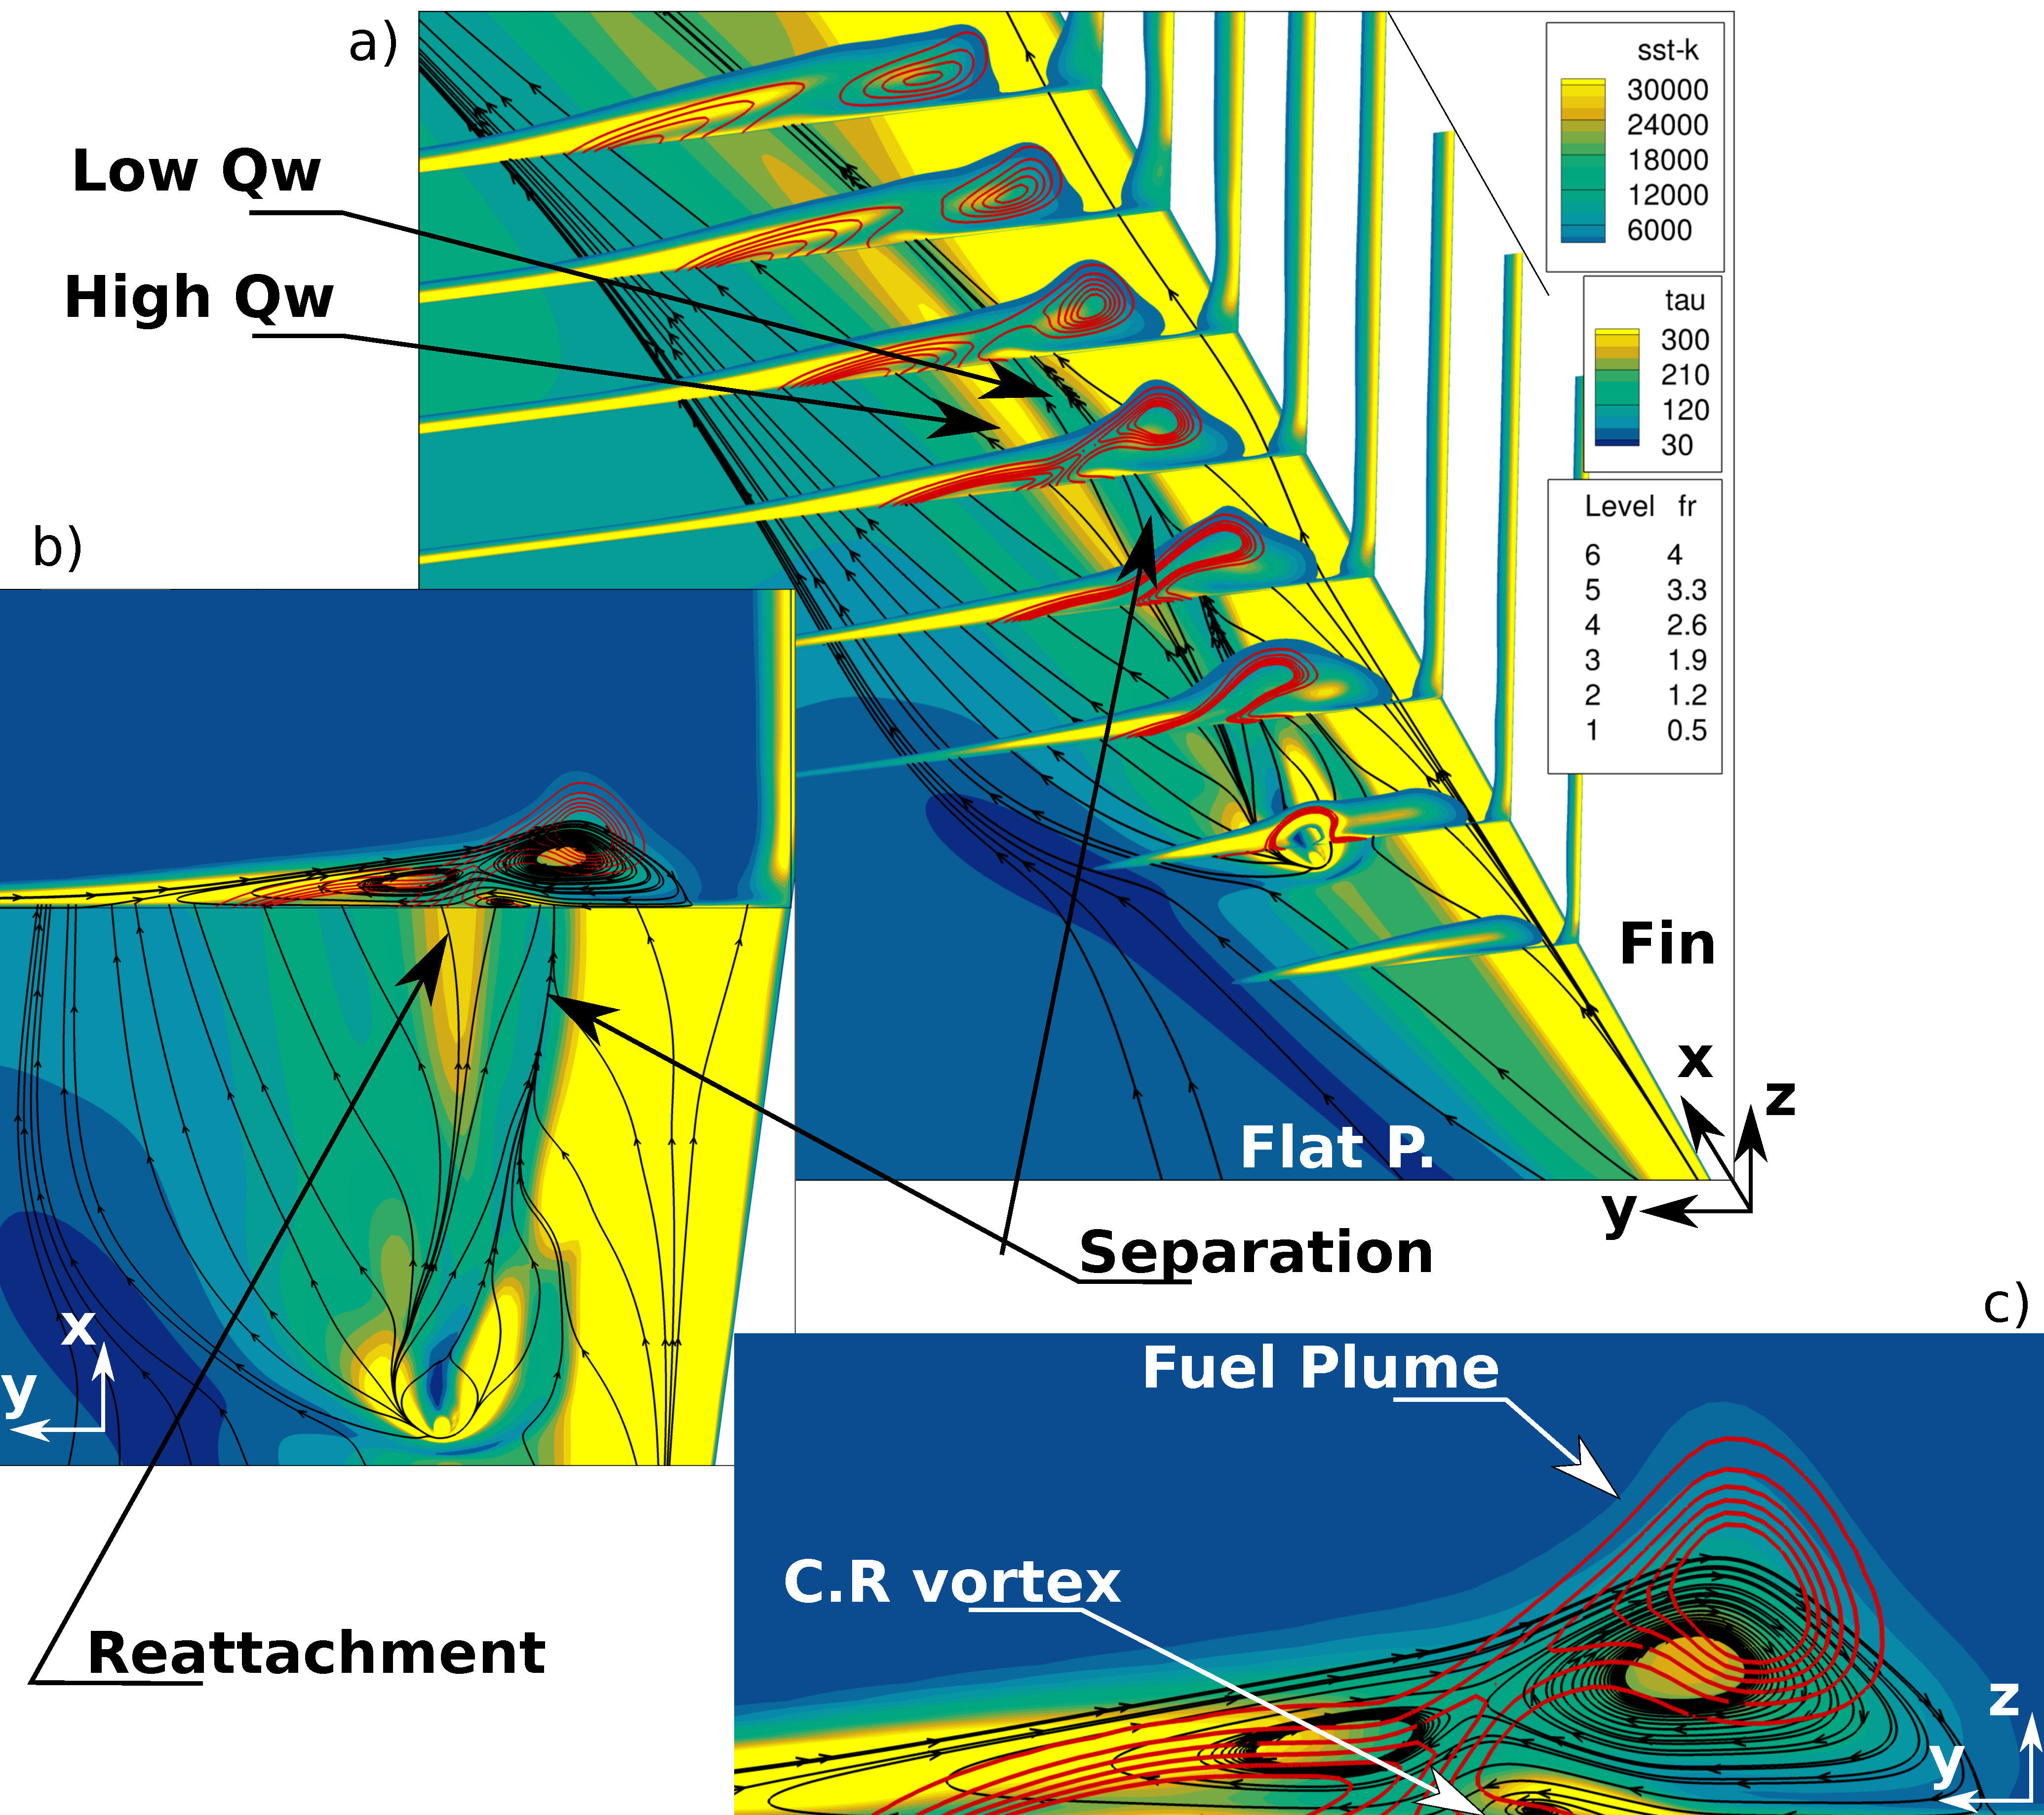
\includegraphics[trim = 0mm 0mm 0mm 0mm, clip, width=0.95\columnwidth,valign=t]{Figures/Flowfield_Experimental_Vred_V2.pdf}
\caption{Flat plate surface: numerical heat flux map with streak-lines. Slices: contours of turbulent kinetic energy, lines of equivalence ratio (red), and surface streamtraces. LP-HI-UF case.}
\label{fig:Exper_Flowf}
\end{figure} 


Despite the previous heat flux overestimation (shown for the NI case), the ability of the numerical method to accurately predict the location and extent of the counter-rotating vortex within the main separation indicates that the macro structures of the 3D flowfield were able to be correctly modeled.


%%%%%%%%%%%%%%%%%%%%
\subsubsection{Upper fin position, Low injection pressure}

The LI-UF case ended up having similar results to the HI-UF case. 
Shown in Fig.~\ref{fig:HeatFluxLPLIUF}, the heat flux peaks are again well predicted and the region away from the fin shock resulted in a good agreement.
Despite these similarities, the low injection case exhibits a larger discrepancy between the numerical and experimental data in the `numerical overestimation zone'. 


%LP_LI_UF
\begin{figure}[!h]
\center
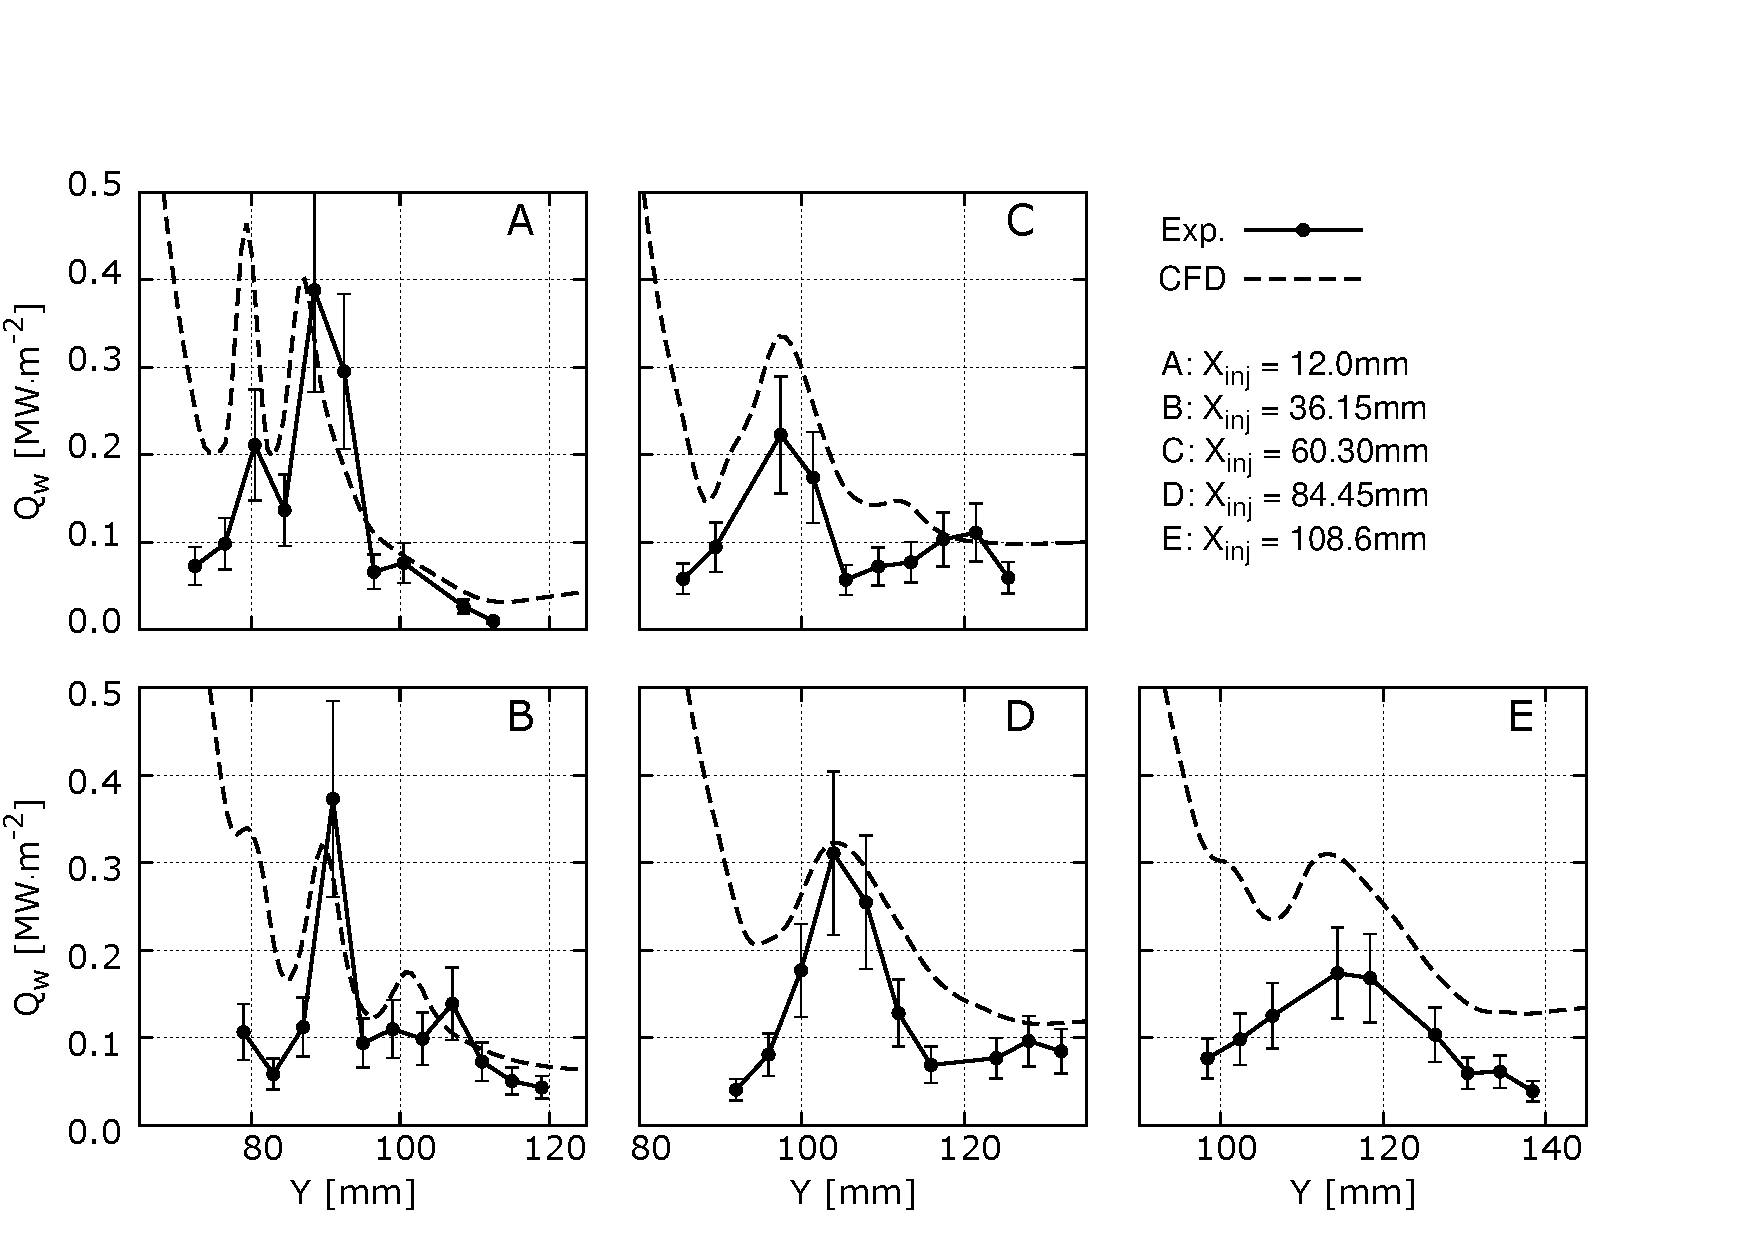
\includegraphics[trim = 0mm 3mm 25mm 25mm, clip, width=0.60\columnwidth,valign=t,fbox]{Figures/Data/LP_LI_UF/GNUP_CFD_GaugesLines_Multi.pdf}
\caption{Numerical and experimental heat transfer data. LI-UF (Case 2 in Table~\ref{tab:T4_Test_Cases})}
\label{fig:HeatFluxLPLIUF}
\end{figure} 
%


For the HI-UF, the injection bow shock has a larger influence the on heat flux, helping to decrease the level of intrinsic error experienced from the `numerical overestimation zone'.
In the LI-UF case shown in Fig.~\ref{fig:HeatFluxLPLIUF}, the lower injection pressure makes the numerical error in the `numerical overestimation zone' more influential on the final results.
This is especially true in lines A and E.
In Line A, the left hand side peak is clearly overestimated due to its proximity to the fin and in Line E, the effect of the injection bow shock is largely dissipated, again increasing relative the effect of the `numerical overestimation zone'.

%%%%%%%%%%%%%%%%%%%%
\subsubsection{Lower fin position, High injection pressure}

The heat flux results for the high injection pressure, low fin position (HI-LF) are presented in Fig.~\ref{fig:HeatFluxLPHILF}.
These lines show a better agreement than the previous cases across the entire domain.
As previously described, the fin shock in the LF position is further from the experimental data acquisition region.
Thus, a smaller spatial area of the `numerical overestimation zone' influences the results. 
This improvement in the correlation between the two results is particularly visible in Line A.
In this line, the experimental data points, even for the values close to the fin wall, are generally within the experimental uncertainty of TFHG readings.
Not only are the location and trend of the heat flux peaks captured, but the heat flux values were able to be accurately predicted as well. 
This improved correlation increases the confidence in both the simulation and numerical results even though previous discrepancies were observed. 


%
%LP_HI_LF
\begin{figure}[!h]
\center
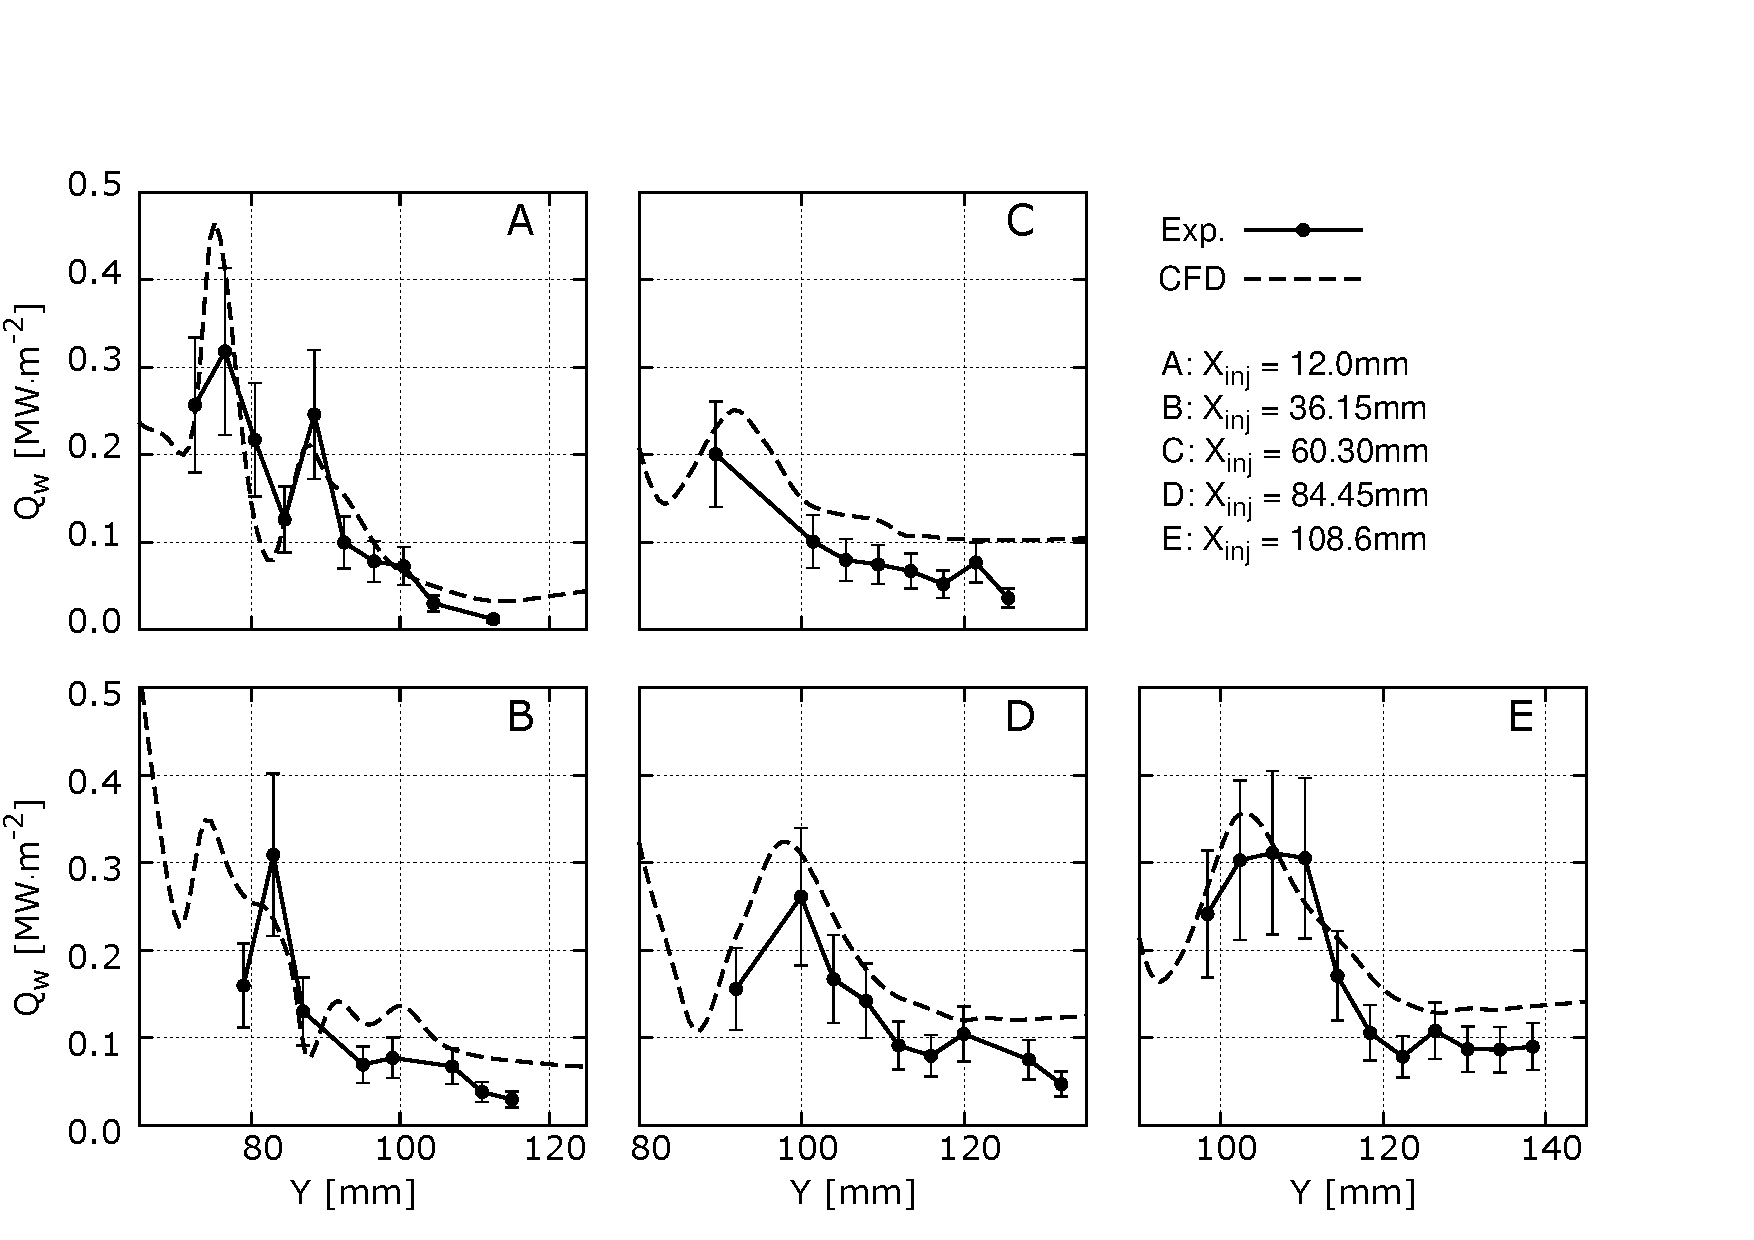
\includegraphics[trim = 0mm 3mm 25mm 25mm, clip, width=0.60\columnwidth,valign=t,fbox]{Figures/Data/LP_HI_LF/GNUP_CFD_GaugesLines_Multi.pdf}
\caption{Numerical and experimental heat transfer data. HI-LF (Case 3 in Table~\ref{tab:T4_Test_Cases})}
\label{fig:HeatFluxLPHILF}
\end{figure} 


%%%%%%%%%%%%%%%%%%%%
\subsubsection{Lower fin position, Low injection pressure}
 
The LI-LF heat flux data is presented in Fig.~\ref{fig:HeatFluxLPLILF}.
Again, thanks to the fin shock sitting further away from the measurement region, the effect of the `numerical overestimation zone' is reduced when compared to the LI-HF case.
Even still, the accuracy of the numerical method is lower than for the equivalent fin position with the higher injection rate (HI-LF).
Similar to the difference shown for the UF cases, this decrease in the accuracy is caused by the reduced effect of the injection bow shock on the measured heat flux values.

%
\begin{figure}[!h]
\center
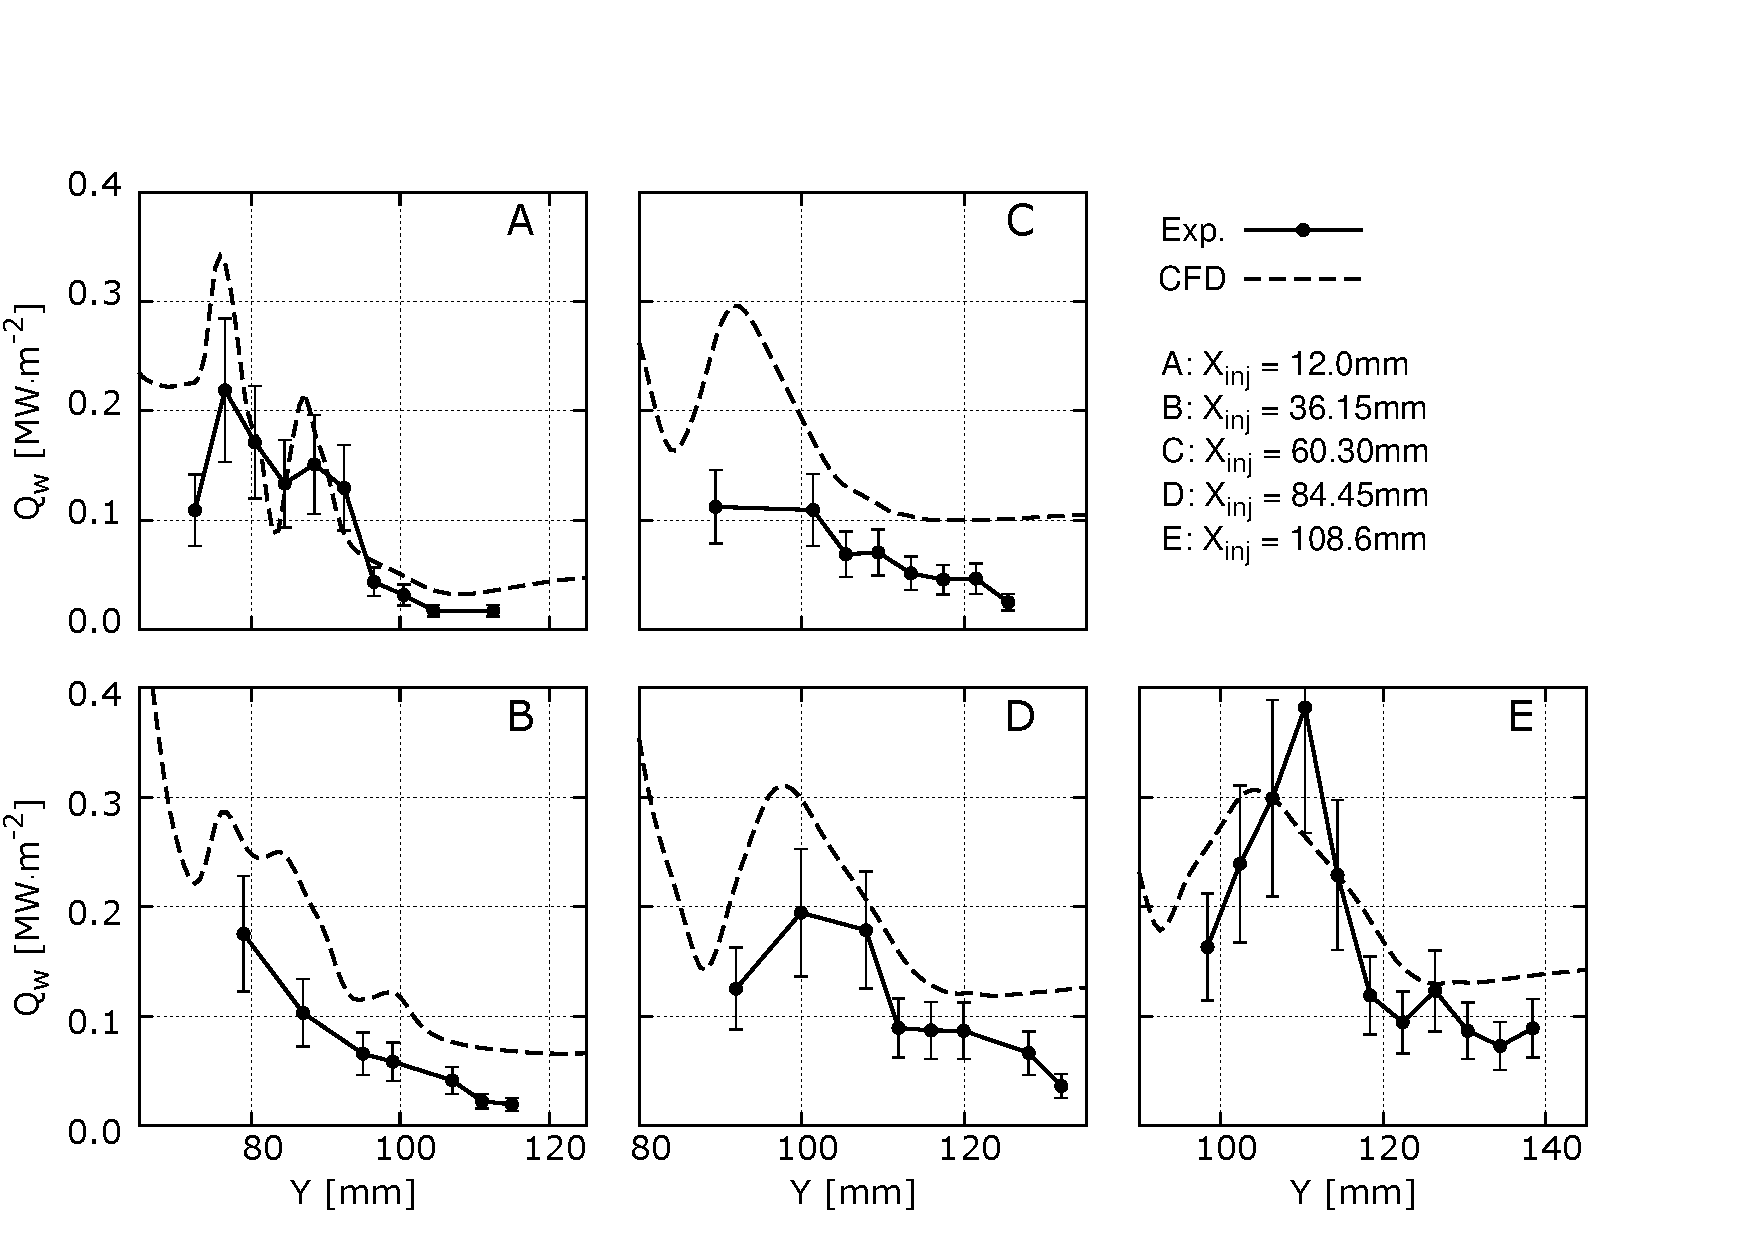
\includegraphics[trim = 0mm 3mm 25mm 25mm, clip, width=0.60\columnwidth,valign=t,fbox]{Figures/Data/LP_LI_LF/GNUP_CFD_GaugesLines_Multi.pdf}
\caption{Numerical and experimental heat transfer data. LI-LF (Case 4 in Table~\ref{tab:T4_Test_Cases})}
\label{fig:HeatFluxLPLILF}
\end{figure} 


%%%%%%%%%%%%%%%%%%%%%%%%%%%%%%%%%%%%%%%%%%%%%%%%%%%%%%%%%%%%%%%%%%%%%%%%%%%%%
\section{Conclusions}

A canonical geometry consisting of a flat plate plus a fin with a compression angle has been used to generate vortices representative of those intrinsically generated by scramjet inlets.
By injecting within this vortex, the vortex-injection interaction and its effect on the heat flux was able to be studied.
Both numerical and experimental results were obtained allowing for the validity of the numerical methodology to accurately predict the experimental results to be assessed.

The vortex measurements with no injection showed a localized region of severe discrepancy near the fin wall between the experimental and numerical results.
This limitation of the numerical methodology was identified as a tendency of the $SST k-\omega$ turbulence model to overpredict the turbulent intensity on the flat plate surface near the fin.
This overestimation of the turbulence intensity was also shown to influence the numerical results for the fueled cases as well.
The effect was found to be less severe as the fin was translated away from the experimental data acquisition gauges.


Despite the limitations of the numerical methodology due to the localized overestimated heat flux, the location of the injection bow shock and secondary counter-rotating vortex was able to be accurately predicted.
Moreover, the correlation between the numerical and experimental results in general increased as you moved in the transverse direction away from the fin.
This increased correlation suggests the that the numerical methodology was able to accurately predict the flow structure but needs improvement in the adjacent to the wall in separation region of the fin shock for both the fueled and unfueled scenarios.


\section{Bibliography}

\begin{thebibliography}{}

%1
\bibitem{SmartTetlow}
Smart, M.~K. \& Tetlow, M.~R., {\it Orbital delivery of small payloads using hypersonic airbreathing propulsion}, J. Spacecraft Rockets, {\bf 46, No.1}, 2009, 117-125.

%2
\bibitem{CookHueter}
Cook, S. \& Hueter, U., {\it NASA's integrated space transportation plan 3rd generation reusable launch vehicle technology update}, Acta Astronautica, 53, 2003, 719-728.

%3
\bibitem{Alvi}
Alvi, F.~S. \& Settles, G.~S., {\it Physical model of the swept shock wave/boundary-layer interaction flowfield}, AIAA Journal, 30, No.9, 1992, 2252-2258.

%4
\bibitem{SpacePlanes_paper2015}
Llobet, J.~R., Jahn, I.~H. \& Gollan, R.~J., {\it Effect of stream-wise Vortices on Scramjets Porthole Injection Mixing}, Proceedings for the 20th AIAA International Space Planes and Hypersonic Systems and Technologies Conference, Glasgow, 2015. 

%5
\bibitem{Llobet_PlumeElongation}
Llobet, J.~R., Gollan, R.~J., \& Jahn, I.~H., {\it Scramjet inlet vortices: its effect on fuel plume elongation and mixing rate}, publication pending.

%6
\bibitem{AFMCpaper2014}
Llobet, J.~R., Barth, J.~E. \& Jahn, I.~H., {\it Vortex Tracking Algorithm for Hypersonic Flow in Scramjets}, 19th AFMC, 8-11 December, Melbourne 2014. Submitted for publication.

%7
\bibitem{Doherty:PhD_Thesis_Scram_M10}
Doherty, L. J. (2013). Experimental Investigation of an Airframe Integrated 3-D Scramjet at a Mach 10 Flight Condition. University of Queensland.

%8
\bibitem{Stalker1966}
Stalker, R~.J., {\it The Free-Pison Shock Tube}, The Aeronautical Quarterly, 1966, 351-370.

%9
\bibitem{Tanimizu:Phd_Thesis}
Tanimizu, K. (2008). Nozzle Optimization Study and Measurements for a Quasi-Axisymmetric Scramjet Model. University of Queensland.

%10
\bibitem{Kirchhartz:PhD_Thesis_Boundary_Combustion}
Kirchhartz, R. M. (2009). Upstream Wall Layer Effects on Drag Reduction with Boundary Layer Combustion. University of Queensland.

%11
\bibitem{RidingsAndrewNoel2015Iops}
Ridings, A. N. (2015). Investigation of pre-combustion shock trains in a scramjet using a shock tunnel at Mach 8 flight conditions. The University of Queensland, School of Mechanical and Mining Engineering.

%12
\bibitem{Chan:Boundary_Layer_Combustion_Perturbation}
Khang, W. C. Y. (2012). Effects of flow non-uniformities on the drag reduction by boundary layer combustion, (August).

%13
\bibitem{Wise_Thesis}
Wise, D., {\it Experimental Investigation of a 3D Scramjet Engine at Hypervelocity Conditions}, PhD thesis, The University of Queensland, 2014.

%14
\bibitem{Stalker_2005}
Stalker, R. J., Paull, A., Mee, D. J., Morgan, R. G., \& Jacobs, P. A. (2005). Scramjets and shock tunnels -The Queensland experience. Progress in Aerospace Sciences, 41, 471–513.

%15
\bibitem{Itoh1999}
Itoh, K., Ueda, S., Komuro, T., Sato, K., Tanno, H., \& Takahashi, M. (1999). Hypervelocity aerothermodynamic and propulsion research using a high enthalpy shock tunnel HIEST. In 9th International Space Planes and Hypersonic Systems and Technologies Conference.

%16
\bibitem{Wise2014b}
Wise, D. J., \& Smart, M. K. (2014). Roughness-Induced Transition of Hypervelocity Boundary Layers. Journal of Spacecraft and Rockets, 51(3), 847–854. https://doi.org/10.2514/1.A32674

%17
\bibitem{Hunt2009}
Hunt, D. C., Paull, A., Boyce, R. R., \& Hagenmaier, M. (2009). Investigation of an Axisymmetric Scramjet Configuration Utilising Inlet Injection and Radical Farming. In 19th International Symposium on Airbreathing Engines (ISABE2009).

%18
\bibitem{JSASS_paper}
Llobet, J.~R., Jahn, I.~H. \& Gollan, R.~J., {\it Effect of vortex-injection interaction on wall heat transfer in a flat plate with fin corner geometry}, Trans. JSASS Aerospace Tech. Japan, Vol.15, No.APISAT-2016, 2017, a17-a26. 

%19
\bibitem{Schultz_Book}
Schultz, D. \& Jones, T., {\it Heat-Transfer Measurements in Short-Duration Hypersonic Facilities}, AGARD-AG-165, North Atlantic Treaty Organization Advisory Group for Aerospace Research and Development, 1973.

%20
\bibitem{nenzfr_manual}
Doherty, L., Zander, F. , Jacobs, P., Gollan, R., Chan, W., \& Kirchhartz, R., {\it NENZF-r: Non-Equilibrium Nozzle Flow, Reloaded. A User Guide.}, Mechanical Engineering Report 2012/08, The University of Queensland School of Mechanical and Mining Engineering, 2012.

%21
\bibitem{Eilmer_TheoryBook}
P.~A. Jacobs, R.~J. Gollan, A.~J. Denman, B.~T. O'Flaherty, D.~F. Potter, P.~J. Petrie-Repar, \& I.~A. Johnston., {\it Eilmer's Theory Book: Basic Models for Gas Dynamics and Thermochemistry.}, Mechanical Engineering Report 2010/09, The University of Queensland School of Mechanical and Mining Engineering, 2010.

%22
\bibitem{Eilmer3UserGuide}
P.~A. Jacobs, \& R.~J. Gollan., {\it The Eilmer3 Code: User Guide and Example Book.}, Mechanical Engineering Report 2008/07, The University of Queensland School of Mechanical and Mining Engineering, 2009.

%23
\bibitem{CEA2}
McBride, B.~J., \& Gordon, S., {\it Computer program for calculation of complex chemical equilibrium	compositions and applications. Part 2: User manual and program description.}, Reference Publication 1311, NASA, 1996.

%24
\bibitem{He_Morgan}
He, Y. \& Morgan, R.~G., {\it Transition of compressible high enthalpy boundary layer
flow over a flat plate}, Aeronautical Journal, 98(972), 2534.



\end{thebibliography}
\end{document}
